%!TEX TS-program = xelatex
%!TEX options = -aux-directory=Debug -shell-escape -file-line-error -interaction=nonstopmode -halt-on-error -synctex=1 "%DOC%"
\documentclass{report}
% Packages

%% Math enhancements
\usepackage{amsmath} % Misc enhancements to math equations
\usepackage{cancel} % Draw diagonal lines and arrows in math equations
\usepackage{mathtools} % Starred versions of amsmath matrix environments; Multiline, cases, gathered environment
\usepackage{chngcntr} % Reset counter within sections
\usepackage{interval} % Format intervals
\intervalconfig{
    soft open fences
}

%% Symbols
\usepackage{amssymb} % Extended symbol collection - also loads amsfonts
\usepackage{stmaryrd} % Extra symbols

%% Fonts
\usepackage{mathrsfs} % Support \mathcal and \mathscr

%% Environments
\usepackage{amsthm} % Use theorems

%% Tables and arrays
\usepackage{booktabs} % Top and bottom rule for tabular
\usepackage{tabularx} % Advanced Tables

%% Lists
\usepackage{enumitem} % Itemize, enumerate, description environments

%% Page layout
\usepackage{geometry} % Page layout customisation
\usepackage{fancyhdr} % Page headers and footers
\usepackage{float} % Float objects such as figures and tables
\usepackage{tcolorbox} % Create boxed environments

%% Text enhancements
\usepackage[none]{hyphenat} % Disable hyphenation of long text
\usepackage{ragged2e} % Text alignment options

%% Referencing
\usepackage{tocbibind} % Adds bibliography to the Table of Contents
\usepackage{url} % Define urls

%% Graphics
\usepackage{graphicx} % Extension to graphics
% \graphicspath{ {./figures/} }

%% Miscellaneous
\usepackage[outputdir=Debug]{minted} % Typeset programming code
\usepackage{siunitx} % SI units package
\usepackage{derivative} % Derivative notation
\usepackage{pdfpages} % Import PDFs into document

\usepackage[hidelinks]{hyperref} % Handle cross-referencing
\usepackage{bookmark} % New bookmark organisation for hyperref

%% Unicode setup
\usepackage[warnings-off={mathtools-colon, mathtools-overbracket}]{unicode-math}
\setmathfont{Latin Modern Math}
\setmathfont[range={bb, bbit}, Scale=MatchUppercase]{TeX Gyre Pagella Math}
\setmathfont[range={\mathcal, \mathbfcal}, StylisticSet=1]{XITS Math}
\setmathfont[range={\mathscr}]{XITS Math}
\setmathfont[range={"2205}]{XITS Math} % chktex 18

% Preamble

%% Misc Commands

%%% Number Sets
\newcommand*{\N}{\mathbb{N}}
\newcommand*{\Z}{\mathbb{Z}}
\newcommand*{\Q}{\mathbb{Q}}
\newcommand*{\I}{\mathbb{I}}
\newcommand*{\R}{\mathbb{R}}
\newcommand*{\C}{\mathbb{C}}

%%% Empty set character
\let\oldemptyset\emptyset
\let\varnothing\relax
\newcommand{\varnothing}{\char"2205} % chktex 18

%%% Contradiction
\newcommand{\contradiction}{
    \hspace{-1em}
	{\hbox{
	\setbox0=\hbox{\(\mkern-3mu{\times}\mkern-3mu\)}
	\setbox1=\hbox to0pt{\hss\copy0\hss}
	\copy0\raisebox{0.5\wd0}{\copy1}\raisebox{-0.5\wd0}{\box1}\box0}}
}

%%% Lines for matrices
\newcommand*{\vertbar}{\rule[-1ex]{0.5pt}{2.5ex}}
\newcommand*{\horzbar}{\rule[.5ex]{2.5ex}{0.5pt}}

%% Paired Delimiters
\DeclarePairedDelimiter{\ceil}{\lceil}{\rceil}
\DeclarePairedDelimiter{\floor}{\lfloor}{\rfloor}
\DeclarePairedDelimiter{\abracket}{\langle}{\rangle}
\DeclarePairedDelimiter{\abs}{\lvert}{\rvert}
\DeclarePairedDelimiter{\norm}{\lVert}{\rVert}

%% Probability Functions
\let\Pr\relax
\DeclareMathOperator{\Pr}{Pr}
\DeclareMathOperator{\E}{E}
\DeclareMathOperator{\Var}{Var}
\DeclareMathOperator{\Cov}{Cov}
\DeclareMathOperator{\Corr}{Corr}

\newcommand{\Perm}[2]{\prescript{#1}{}{P}_{#2}}

%% Hyperbolic Functions
\DeclareMathOperator{\arcsinh}{arcsinh}
\DeclareMathOperator{\arccosh}{arccosh}
\DeclareMathOperator{\arctanh}{arctanh}
\DeclareMathOperator{\arccoth}{arccoth}
\DeclareMathOperator{\arcsech}{arcsech}
\DeclareMathOperator{\arccsch}{arccsch}

%% Linear Algebra
%%% Augmented matrices
\makeatletter
\renewcommand*\env@matrix[1][*\c@MaxMatrixCols c]{%
  \hskip -\arraycolsep
  \let\@ifnextchar\new@ifnextchar
  \array{#1}}
\makeatother

%%% Operators
\let\det\relax
\DeclareMathOperator{\det}{det}
\DeclareMathOperator{\Tr}{Tr}
\DeclareMathOperator{\diag}{diag}
\DeclareMathOperator{\adj}{adj}

\DeclareMathOperator{\vspan}{span}
\DeclareMathOperator{\vref}{ref}
\DeclareMathOperator{\vrref}{rref}

\DeclareMathOperator{\vrank}{rank}
\DeclareMathOperator{\vnull}{null}

\DeclareMathOperator{\proj}{proj}

\DeclareMathOperator{\vim}{im}
\DeclareMathOperator{\vcoim}{coim}
\DeclareMathOperator{\vker}{ker}
\DeclareMathOperator{\vcoker}{coker}

\newcommand{\columnspace}[1]{\mathcal{C}\left(\symbf{#1}\right)}
\newcommand{\rowspace}[1]{\mathcal{C}\left(\symbf{#1}^{\top}\right)}
\newcommand{\nullspace}[1]{\mathcal{N}\left(\symbf{#1}\right)}
\newcommand{\leftnullspace}[1]{\mathcal{N}\left(\symbf{#1}^{\top}\right)}

%% Additional operators
\DeclareMathOperator{\erf}{erf}

% Theorems
\theoremstyle{definition}
\newtheorem{definition}{Definition}[section]

\theoremstyle{plain}
\newtheorem{theorem}{Theorem}[subsection]
\newtheorem{corollary}{Corollary}[theorem]
\newtheorem{lemma}{Lemma}[theorem]
\newtheorem{axiom}{Axiom}

\theoremstyle{remark}
\newtheorem{remark}{Remark}
\newtheorem{note}{Note}[subsection]
\newtheorem*{statement}{Statement}

\newenvironment{examples}[1][Examples]{\let\qed\relax\proof[#1]\mbox{}\\*}{\endproof}
\newenvironment{question}[1][Question]{\let\qed\relax\proof[#1]\mbox{}\\*}{\endproof}
\newenvironment{solution}[1][Solution]{\let\qed\relax\proof[#1]\mbox{}\\*}{\endproof}

\newenvironment{proofcase}[1]{\proof[Case #1]\mbox{}}{\endproof}

%% Box styles
\tcbuselibrary{skins}
\newtcolorbox{tcolorboxlarge}[1][]{
    skin=enhanced,
    boxrule=0pt,
    frame hidden,
    sharp corners,
    borderline west={0.5pt}{0pt}{black},
    borderline east={0.5pt}{0pt}{black},
    enlarge left by=10pt,
    width=\linewidth-20pt,
    opacityback=0,
    coltitle=black,
    fonttitle=\large\bfseries,
    #1
}

\newtcolorbox{tcolorboxcols}[1][]{
    skin=enhanced,
    boxrule=0pt,
    frame hidden,
    sharp corners,
    borderline west={0.5pt}{0pt}{black},
    opacityback=0,
    coltitle=black,
    fonttitle=\large\bfseries,
    #1
}

%% Reset counter within subsections
\counterwithin*{equation}{section}
\counterwithin*{equation}{subsection}
\counterwithin*{remark}{subsection}

%% Page layout setup
\pagestyle{fancy}
\setlength\headheight{24pt}
\setlength\parindent{0pt} % Indent first line of new paragraphs


% Additional packages & macros
\usepackage{xcolor}
\newcommand{\keyword}[1]{\textcolor[rgb]{0.00,0.50,0.00}{\textbf{#1}}}
\newcommand{\keywordinline}[1]{\textcolor[rgb]{0.00,0.50,0.00}{\textbf{\mintinline{ca65}{#1}}}}

\setminted{
    escapeinside=||,
    linenos,
    frame=lines,
    breakanywhere
}

\usepackage{subcaption}
\usepackage{multicol}
\usepackage{multirow}

% Header and footer
\newcommand{\unitName}{Microprocessors and Digital Systems}
\newcommand{\unitTime}{Semester 2, 2022}
\newcommand{\unitCoordinator}{Dr Mark Broadmeadow}
\newcommand{\documentAuthors}{Tarang Janawalkar}

\fancyhead[L]{\unitName}
\fancyhead[R]{\parbox[t]{0.6\textwidth}{\raggedleft\leftmark\strut}}
\fancyfoot[C]{\thepage}

% Copyright
\usepackage[
    type={CC},
    modifier={by-nc-sa},
    version={4.0},
    imagewidth={5em},
    hyphenation={raggedright}
]{doclicense}

\date{}

\begin{document}
%
\begin{titlepage}
    \vspace*{\fill}
    \begin{center}
        \LARGE{\textbf{\unitName}} \\[0.1in]
        \normalsize{\unitTime} \\[0.2in]
        \normalsize\textit{\unitCoordinator} \\[0.2in]
        \documentAuthors
    \end{center}
    \vspace*{\fill}
    \doclicenseThis
    \thispagestyle{empty}
\end{titlepage}
\newpage
%
\tableofcontents
\newpage
%
\part{Microcontrollers}
\chapter{Microcontroller Fundamentals}
\section{Architecture of a Computer}
\begin{definition}[Computer]
    A computer is a digital electronic machine that can be programmed to carry
    out sequences of arithmetic or logical operations (computation) automatically.
\end{definition}
\begin{definition}[Control unit]
    The control unit interprets the instructions and decides what actions to take.
\end{definition}
\begin{definition}[Arithmetic logic unit]
    The arithmetic logic unit (ALU) performs computations required by the control unit.
\end{definition}
\section{Microprocessors \& Microcontrollers}
While a microcontroller puts the CPU and all peripherals onto the same chip,
a microprocessor houses a more powerful CPU on a single chip that connects to external peripherals.
The peripherals include memory, I/O, and control units.
The QUTy uses a microcontroller called ATtiny1626, that are within a family of microcontrollers called AVRs.
\section{ATtiny1626 Microcontroller}
The ATtiny1626 microcontroller has the following features:
\begin{itemize}
    \item CPU:\@ AVR Core (AVRxt variant)
    \item Memory:\@
          \begin{itemize}
              \item Flash memory (16KB) used to store program instructions in memory
              \item SRAM (2KB) used to store data in memory
              \item EEPROM (256B)
          \end{itemize}
    \item Peripherals:\@ Implemented in hardware (part of the chip) in order to offload complexity
\end{itemize}
\subsection{Flash Memory}
\begin{itemize}
    \item Non-volatile --- memory is not lost when power is removed
    \item Inexpensive
    \item Slower than SRAM
    \item Can only erase in large chunks
    \item Typically used to store program data
    \item Generally read-only. Programmed via an external tool, which is loaded once and remains static during the lifetime of the program
    \item Writing is slow
\end{itemize}
\subsection{SRAM}
\begin{itemize}
    \item Volatile --- memory is lost when power is removed
    \item Expensive
    \item Faster than flash memory and is used to store variables and temporary data
    \item Can access individual bytes (large chunk erases are not required)
\end{itemize}
\subsection{EEPROM}
\begin{itemize}
    \item Older technology
    \item Expensive
    \item Non-volatile
    \item Can erase individual bytes
\end{itemize}
\section{AVR Core}
\begin{definition}[Computer program]
    A computer program is a sequence or set of instructions in a programming language
    for a computer to execute.
\end{definition}
The main function of the AVR Core Central Processing Unit (CPU) is to ensure correct program execution.
The CPU must, therefore, be able to access memory, perform calculations, control peripherals, and handle interrupts.
Some key characteristics of the AVR Core are:
\begin{itemize}
    \item 8-bit Reduced Instruction Set Computer (RISC)
    \item 32 working registers (R0 to R31)
    \item Program Counter (PC) --- location in memory where the program is stored
    \item Status Register (SREG) --- stores key information from calculations performed by the ALU (i.e., whether a result is negative)
    \item Stack Pointer --- temporary data that doesn't fit into the registers
    \item 8-bit core --- all data, registers, and operations, operate within 8-bits
\end{itemize}
\section{Status Register}
The status register is a 8-bit register that stores the result of the last operation performed by the ALU.
It has the following flags:
\begin{itemize}
    \item[\textbf{C}] Carry Flag
    \item[\textbf{Z}] Zero Flag
    \item[\textbf{N}] Negative Flag
    \item[\textbf{V}] Two's Complement Overflow Flag
    \item[\textbf{S}] Sign Flag
    \item[\textbf{H}] Half Carry Flag
    \item[\textbf{T}] Transfer Bit
    \item[\textbf{I}] Global Interrupt Enable Bit
\end{itemize}
\section{Program Execution}
At the time of reset, PC = 0. The following steps are then performed:
\begin{enumerate}
    \item Fetch instruction (from memory)
    \item Decode instruction (decode binary instruction)
    \item Execute instruction:
          \begin{itemize}
              \item Execute an operation
              \item Store data in data memory, the ALU, a register, or update the stack pointer
          \end{itemize}
    \item Store result
    \item Update PC (move to next instruction or if instruction is longer than 1 word, increment twice. The program can also move to another point in the program that has an address \(k\), through jumps.)
\end{enumerate}
This is illustrated in the following figure:
\begin{figure}[H]
    \centering
    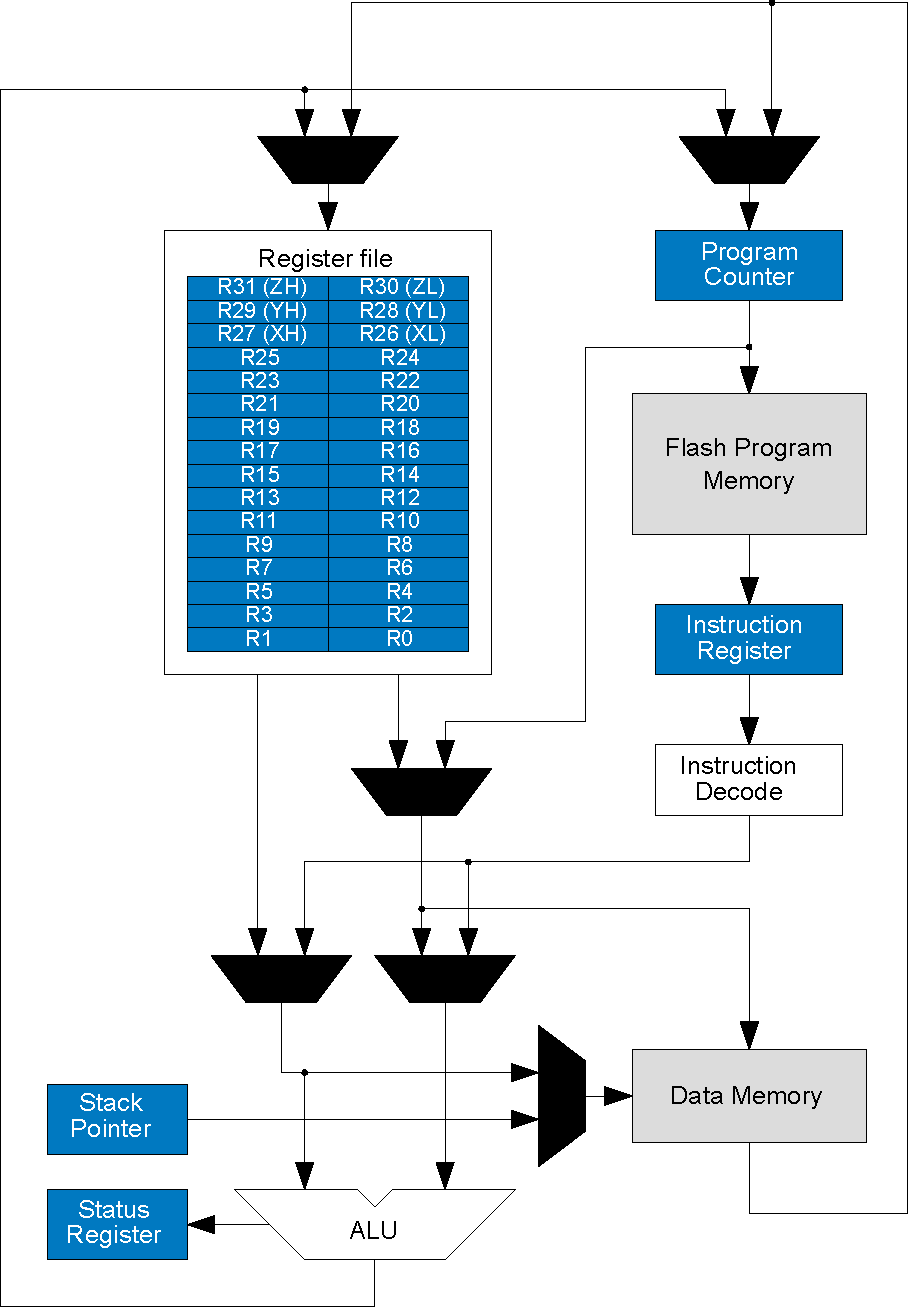
\includegraphics[height = 12cm, keepaspectratio = true]{figures/AVR_CPU.pdf}
    \caption{Program execution on the ATtiny1626.} % \label{}
\end{figure}
\section{Instructions}
\begin{itemize}
    \item The CPU understands and can execute a limited set of instructions --- \textasciitilde88 unique instructions for the ATtiny1626
    \item Instructions are encoded in program memory as opcodes. Most instructions are two bytes long, but some instructions are four bytes long
    \item The AVR Instruction Set Manual describes all of the available instructions, and how they are translated into opcodes
    \item Instructions fall loosely into five categories:
          \begin{itemize}
              \item Arithmetic and logic --- ALU
              \item Change of flow --- jumping to different sections of the code or making decisions
              \item Data transfer --- moving data in/out of registers, into the data space, or into RAM
              \item Bit and bit-test --- looking at data in registers (which bits are set or not set)
              \item Control --- changing what the CPU is doing
          \end{itemize}
\end{itemize}
\section{Interacting with memory and peripherals}
\begin{itemize}
    \item The CPU interacts with both memory and peripherals via the data space
    \item From the perspective of the CPU, the data space is single large array of
          locations that can be read from, or written to, using an address
    \item We control peripherals by reading from, and writing to, their registers
    \item Each peripheral register is assigned a unique address in the data space
    \item When a peripheral is accessed in this manner we refer to it as being
          memory mapped, as we access them as if they were normal memory
    \item Different devices, peripherals and memory can be included in a memory map
          (and sometimes a device can be accessed at multiple different addresses)
\end{itemize}
\section{Assembly code}
\begin{itemize}
    \item The opcodes placed into program memory are called
          machine code (i.e., code the machine operates on directly)
    \item We don't write machine code directly as it is:
          \begin{itemize}
              \item Not human readable
              \item Prone to errors (swapping a single bit can completely change the operation)
          \end{itemize}
    \item Instead we can write instructions directly in assembly code
    \item We use instruction mnemonics to specify each instruction:\@ \keywordinline{ldi}, \keywordinline{add}, \keywordinline{sts}, \mintinline{ca65}{jmp}, \dots
    \item An assembler takes assembly code and translates it into opcodes that can
          be loaded into program memory
\end{itemize}
\chapter{Digital Representations and Operations}
\section{Digital Systems}
A \textbf{bit}\footnote{The term \textit{bit} comes from \textbf{b}inary dig\textbf{it}.}
is the most basic unit of information in a digital system.
A bit encodes a logical state with one of two possible values (i.e., binary).
These states are often referred to as:
\begin{itemize}
    \item true, false
    \item high, low (voltage states)
    \item on, off (logical states)
    \item set, reset
    \item 1, 0
\end{itemize}
A sequence of \textit{eight} bits is known as a \textbf{byte}, and it is the most
common representation of data in digital systems.
A sequence of \textit{four} bits is known as a \textbf{nibble}.
A sequence of \(n\) bits can represent up to \(2^n\) states.
\section{Representation}
\subsection{Binary Representation}
The \textbf{binary system} is a base-2 system that uses a sequence of bits to represent a number.
Bits are written right-to-left from \textbf{least significant} to \textbf{most significant} bit.

The first bit is the ``most significant'' bit because it is associated with the highest value in the sequence (coefficient of the highest power of two).
\begin{itemize}
    \item The \textbf{least significant bit} (LSB) is at bit index 0.
    \item The \textbf{most significant bit} (MSB) is at bit index \(n - 1\) in an \(n\)-bit sequence.
\end{itemize}
\begin{align*}
    0000_2 & = 0 & 0100_2 & = 4 & 1000_2 & = 8  & 1100_2 = 12 \\
    0001_2 & = 1 & 0101_2 & = 5 & 1001_2 & = 9  & 1101_2 = 13 \\
    0010_2 & = 2 & 0110_2 & = 6 & 1010_2 & = 10 & 1110_2 = 14 \\
    0011_2 & = 3 & 0111_2 & = 7 & 1011_2 & = 11 & 1111_2 = 15
\end{align*}
The subscript 2 indicates that the number is represented using a base-2 system.
\subsection{Hexadecimal Representation}
The \textbf{hexadecimal system} (hex) is a base-16 system. As we need 16 digits in this system, we use the letters A to F to represent digits 10 to 15.

Hex is a convenient notation when working with digital systems as each hex digit maps to a nibble.
\begin{align*}
    0_{16} & = 0000_2 & 4_{16} & = 0100_2 & 8_{16} & = 1000_2 & C_{16} = 1100_2 \\
    1_{16} & = 0001_2 & 5_{16} & = 0101_2 & 9_{16} & = 1001_2 & D_{16} = 1101_2 \\
    2_{16} & = 0010_2 & 6_{16} & = 0110_2 & A_{16} & = 1010_2 & E_{16} = 1110_2 \\
    3_{16} & = 0011_2 & 7_{16} & = 0111_2 & B_{16} & = 1011_2 & F_{16} = 1111_2
\end{align*}
\subsection{Numeric Literals}
When a fixed value is declared directly in a program, it is referred to as a \textbf{literal}.
Prefixes denote various bases:
\begin{itemize}
    \item \textbf{Binary} notation requires the prefix \mintinline{ca65}{0b}
    \item \textbf{Decimal} notation does not require prefixes
    \item \textbf{Hexadecimal} notation requires the prefix \mintinline{ca65}{0x}
\end{itemize}
For example, \mintinline{ca65}{0x80 |=| 0b10000000 |=| 128}. % chktex 29
\section{Unsigned Integers}
The \textbf{unsigned integers} represent the set of counting (natural) numbers, starting at 0.
In the \textbf{decimal system} (base-10), the unsigned integers are encoded using a sequence of decimal digits (0--9).

The decimal system is a \textbf{positional numeral system}, where the contribution of each digit is determined by its position.
For example,
\begin{align*}
    278_{10} & = 2 \times 10^2 &  & + 7 \times 10^1 &  & + 8 \times 10^0 \\
             & = 2 \times 100  &  & + 7 \times 10   &  & + 8 \times 1    \\
             & = 200           &  & + 70            &  & + 8             \\
\end{align*}
In the \textbf{binary system} (base-2) the unsigned integers are encoded using a sequence of binary digits (0--1)
in the same manner. For example,
\begin{align*}
    10101_2 & = 1 \times 2^4 &  & + 0 \times 2^3 &  & + 1 \times 2^2 &  & + 0 \times 2^1 &  & + 1 \times 2^0 \\
            & = 1 \times 16  &  & + 0 \times 8   &  & + 1 \times 4   &  & + 0 \times 2   &  & + 1 \times 1   \\
            & = 16           &  & + 0            &  & + 4            &  & + 0            &  & + 1            \\
            & = 21_{10}
\end{align*}
The range of values an \(n\)-bit binary number can hold when encoding an unsigned integer is 0 to \(2^n - 1\).
\begin{table}[H]
    \centering
    \begin{tabular}{c c}
        \toprule
        \textbf{No.\ of Bits} & \textbf{Range}                        \\
        \midrule
        8                     & \(0\)--\(255\)                        \\
        16                    & \(0\)--\(\num{65535}\)                \\
        32                    & \(0\)--\(\num{4294967295}\)           \\
        64                    & \(0\)--\(\num{18446744073709551615}\) \\
        \bottomrule
    \end{tabular}
    \caption{Range of available values in binary representations.} % \label{}
\end{table}
\section{Signed Integers}
Signed integers are used to represent integers that can be positive or negative.
The following representations allow us to encode negative integers using a sequence of binary bits:
\begin{itemize}
    \item Sign-magnitude
    \item One's complement
    \item Two's complement (most common)
\end{itemize}
\subsection{Sign-Magnitude}
In sign-magnitude representation, the most significant bit encodes the sign of the
integer. In an 8-bit sequence, the remaining 7-bits are used to
encode the value of the bit.
\begin{itemize}
    \item If the sign bit is 0, the remaining bits represent a positive value,
    \item If the sign bit is 1, the remaining bits represent a negative value.
\end{itemize}
As the sign bit consumes one bit from the sequence, the range of values that can be
represented by an \(n\)-bit sign-magnitude encoded bit sequence is:
\begin{equation*}
    -\left( 2^{n - 1} - 1 \right) \text{ to } 2^{n - 1} - 1
\end{equation*}
For 8-bit sequences, this range is: \(-127\) to \(127\).
This presents several issues:
\begin{enumerate}
    \item There are two ways to represent zero: \mintinline{ca65}{0b10000000 |=| 0}, or \mintinline{ca65}{0b00000000 |=| -0}.
    \item Arithmetic and comparison requires inspecting the sign bit
    \item The range is reduced by 1 (due to the redundant zero representation)
\end{enumerate}
\subsection{One's Complement}
In one's complement representation, a negative number is represented by
inverting the bits of a positive number (i.e., \(0 \to 1\) and \(1 \to 0\)).
The range of values are still the same:
\begin{equation*}
    -\left( 2^{n - 1} - 1 \right) \text{ to } 2^{n - 1} - 1
\end{equation*}
however, this representation tackles the second problem in the previous representation as
addition is performed via standard binary addition with \textit{end-around carry} (carry bit is added onto result).
\begin{equation*}
    a - b = a + \left( \text{\textasciitilde} b \right) + C.
\end{equation*}
\subsection{Two's Complement}
In two's complement representation, the most significant bit encodes a negative weighting of
\(-2^{n - 1}\). For example, in 8-bit sequences, index-7 represents a value of \(-128\).
The two's complement is calculated by adding 1 to the one's complement.
The range of values are:
\begin{equation*}
    -2^{n - 1} \text{ to } 2^{n - 1} - 1
\end{equation*}
This representation is more efficient than the previous because \mintinline{ca65}{0} has a single representation
and subtraction is performed by adding the two's complement of the subtrahend.
\begin{equation*}
    a - b = a + \left( \text{\textasciitilde} b + 1 \right).
\end{equation*}
\section{Logical Operators}
\subsection{Boolean Functions}
A Boolean function is a function whose arguments and results assume values
from a two-element set, (usually \(\left\{ 0,\: 1 \right\}\) or \mintinline{text}{{false, true}}).
These functions are also referred to as \textit{logical functions} when they operate on bits.
The most common logical functions available to microprocessors and most programming languages are:
\begin{itemize}
    \item Negation: \keywordinline{NOT} \(a\), \textasciitilde\(a\), \(\overline{a}\)
    \item Conjunction: \(a\) \mintinline{ca65}{AND} \(b\), \(a\) \mintinline{ca65}{&} \(b\), \(a \cdot b\), \(a \land b\)
    \item Disjunction: \(a\) \keywordinline{OR} \(b\), \(a\) \mintinline{ca65}{|\vert|} \(b\), \(a + b\), \(a \lor b\)
    \item Exclusive disjunction: \(a\) \keywordinline{XOR} \(b\), \(a\) \mintinline{ca65}{^} \(b\), \(a \oplus b\)
\end{itemize}
By convention, we map a bit value of \mintinline{ca65}{0} to \mintinline{ca65}{false}, and a bit value of \mintinline{ca65}{1} to \mintinline{ca65}{true}.
\subsection{Negation}
A unary operator used to \textbf{invert} a bit.
\begin{table}[H]
    \centering
    \begin{tabular}{c c}
        \toprule
        \textbf{\(a\)} & \keywordinline{NOT} \(a\) \\
        \midrule
        0              & 1                         \\
        1              & 0                         \\
        \bottomrule
    \end{tabular}
\end{table}
\subsection{Conjunction}
\mintinline{ca65}{AND} is a binary operator whose output is true if \textbf{both} inputs are \textbf{true}.
\begin{table}[H]
    \centering
    \begin{tabular}{c c c}
        \toprule
        \textbf{\(a\)} & \textbf{\(b\)} & \textbf{\(a\) \mintinline{ca65}{AND} \(b\)} \\
        \midrule
        0              & 0              & 0                                           \\
        0              & 1              & 0                                           \\
        1              & 0              & 0                                           \\
        1              & 1              & 1                                           \\
        \bottomrule
    \end{tabular}
\end{table}
\subsection{Disjunction}
\keywordinline{OR} is a binary operator whose output is true if \textbf{either} input is \textbf{true}.
\begin{table}[H]
    \centering
    \begin{tabular}{c c c}
        \toprule
        \textbf{\(a\)} & \textbf{\(b\)} & \(a\) \keywordinline{OR} \(b\) \\
        \midrule
        0              & 0              & 0                              \\
        0              & 1              & 1                              \\
        1              & 0              & 1                              \\
        1              & 1              & 1                              \\
        \bottomrule
    \end{tabular}
\end{table}
\subsection{Exclusive Disjunction}
\keywordinline{XOR} (Exclusive \keywordinline{OR}) is a binary operator whose output is true if \textbf{only one} input is \textbf{true}.
\begin{table}[H]
    \centering
    \begin{tabular}{c c c}
        \toprule
        \textbf{\(a\)} & \textbf{\(b\)} & \(a\) \keywordinline{XOR} \(b\) \\
        \midrule
        0              & 0              & 0                               \\
        0              & 1              & 1                               \\
        1              & 0              & 1                               \\
        1              & 1              & 0                               \\
        \bottomrule
    \end{tabular}
\end{table}
\subsection{Bitwise Operations}
When applying logical operators to a sequence of bits, the operation is performed in a \textbf{bitwise} manner. The result of each operation is stored in the corresponding bit index also.
\section{Bit Manipulation}
Often we need to modify individual bits within a byte, \textbf{without} modifying other bits.
This is accomplished by performing a bitwise operation on the byte using a \textbf{bit mask} or \textbf{bit field}.

These operations can:
\begin{itemize}
    \item \textbf{Set} specific bits (change value to \mintinline{ca65}{1})
    \item \textbf{Clear} specific bits (change value to \mintinline{ca65}{0})
    \item \textbf{Toggle} specific bits (change values from \(0 \to 1\), or \(1 \to 0\))
\end{itemize}
\subsection{Setting Bits}
To \textbf{set} a bit, we take the bitwise \keywordinline{OR} of the byte, with a bit mask
that has a \textbf{1} in each position where the bit should be set.
\begin{figure}[H]
    \centering
    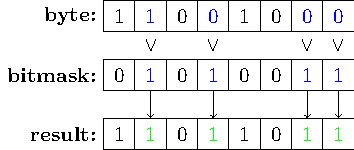
\includegraphics[height = 4cm, keepaspectratio = true]{figures/bit_set.pdf}
    \caption{Setting bits using the logical or.} % \label{}
\end{figure}
\subsection{Clearing Bits}
To \textbf{clear} a bit, we take the bitwise \mintinline{ca65}{AND} of the byte, with a bit mask
that has a \textbf{0} in each position where the bit should be cleared.
\begin{figure}[H]
    \centering
    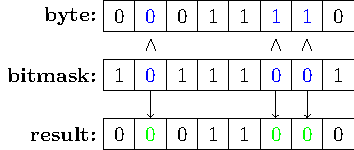
\includegraphics[height = 4cm, keepaspectratio = true]{figures/bit_clear.pdf}
    \caption{Clearing bits using the logical and.} % \label{}
\end{figure}
\subsection{Toggling Bits}
To \textbf{toggle} a bit, we take the bitwise \keywordinline{XOR} of the byte, with a bit mask
that has a \textbf{1} in each position where the bit should be toggled.
\begin{figure}[H]
    \centering
    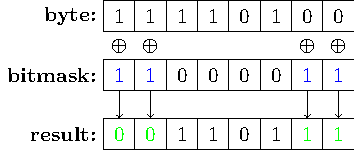
\includegraphics[height = 4cm, keepaspectratio = true]{figures/bit_toggle.pdf}
    \caption{Toggling bits using the logical exclusive or.} % \label{}
\end{figure}
Other bitwise operations act on the entire byte.
\begin{itemize}
    \item One's complement (bitwise \keywordinline{NOT})
    \item Two's complement (bitwise \keywordinline{NOT} + 1)
    \item Shifts
          \begin{itemize}
              \item Logical
              \item Arithmetic (for signed integers)
          \end{itemize}
    \item Rotations
\end{itemize}
\subsection{One's Complement}
The one's complement of a byte inverts every bit in the operand. This is done by
taking the bitwise \keywordinline{NOT} of the byte.
Similarly, we can subtract the byte from \mintinline{ca65}{0xFF} to get the one's complement.
\subsection{Two's Complement}
The two's complement of a byte is the one's complement of the byte plus one.
Therefore, we can apply take the bitwise \keywordinline{NOT} of the byte, and then add one to it.
\subsection{Shifts}
Shifts are used to move bits within a byte. In many programming languages this is represented by two greater than \mintinline{ca65}{>>} or two less than \mintinline{ca65}{<<} characters.
\begin{equation*}
    a \gg s
\end{equation*}
shifts the bits in \(a\) by \(s\) places to the right while adding \mintinline{ca65}{0}'s to the MSB.\
\begin{figure}[H]
    \centering
    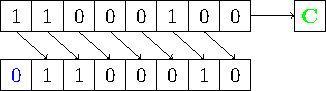
\includegraphics[height = 2cm, keepaspectratio = true]{figures/logical_right_shift.pdf}
    \caption{Right shift using \mintinline{ca65}{lsr} in AVR Assembly.} % \label{}
\end{figure}
Similarly
\begin{equation*}
    a \ll s
\end{equation*}
shifts the bits in \(a\) by \(s\) places to the left while adding \mintinline{ca65}{0}'s to the LSB.\
\begin{figure}[H]
    \centering
    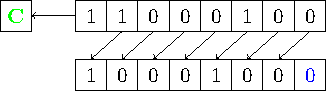
\includegraphics[height = 2cm, keepaspectratio = true]{figures/logical_left_shift.pdf}
    \caption{Left shift using \keyword{\ttfamily{lsl}} in AVR Assembly.} % \label{}
\end{figure}
When using signed integers, the arithmetic shift is used to preserve the value of the sign bit when shifting.
\begin{figure}[H]
    \centering
    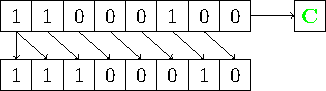
\includegraphics[height = 2cm, keepaspectratio = true]{figures/arithmetic_right_shift.pdf}
    \caption{Arithmetic right shift using \keyword{\ttfamily{asr}} in AVR Assembly.} % \label{}
\end{figure}
Left shifts are used to multiply numbers by 2, whereas right shifts are used to divide numbers by 2 (with truncation).
\subsection{Rotations}
Rotatations are used to shift bits with a carry from the previous instruction.
\begin{figure}[H]
    \centering
    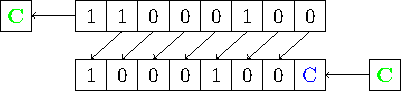
\includegraphics[height = 2cm, keepaspectratio = true]{figures/rotate_left.pdf}
    \caption{Rotate left using \mintinline{ca65}{rol} in AVR Assembly.} % \label{}
\end{figure}
\begin{figure}[H]
    \centering
    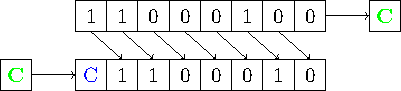
\includegraphics[height = 2cm, keepaspectratio = true]{figures/rotate_right.pdf}
    \caption{Rotate right using \mintinline{ca65}{ror} in AVR Assembly.} % \label{}
\end{figure}
Here the blue bit is carried from the previous instruction, and the carry bit is updated
to the value of the bit that was shifted out.
Rotations are used to perform multi-byte shifts and arithmetic operations.
\section{Arithmetic Operations}
\subsection{Addition}
Addition is performed using the same process as decimal addition except we only use two digits, 0 and 1.
\begin{enumerate}
    \item \mintinline{ca65}{0b0 + 0b0 = 0b0}
    \item \mintinline{ca65}{0b0 + 0b1 = 0b1}
    \item \mintinline{ca65}{0b1 + 0b1 = 0b10}
\end{enumerate}
When adding two 1's, we carry the result into the next bit position as we would with a 10 in decimal addition.
In AVR Assembly, we can use the \keywordinline{add} instruction to add two bytes. The following
example adds two bytes.
\begin{minted}{ca65}
; Accumulator
|\keyword{ldi}| r16, 0

; First number
|\keyword{ldi}| r17, 29
|\keyword{add}| r16, 17 ; R16 <- R16 + R17 = 0 + 29 = 29

; Second number
|\keyword{ldi}| r17, 118
|\keyword{add}| r16, 17 ; R16 <- R16 + R17 = 29 + 118 = 147
\end{minted}
Below is a graphical illustration of the above code.
\begin{figure}[H]
    \centering
    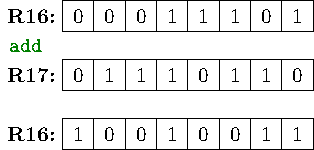
\includegraphics[height = 3cm, keepaspectratio = true]{figures/add.pdf}
    \caption{Overflow addition using \keyword{\ttfamily{add}} in AVR Assembly.} % \label{}
\end{figure}
\subsection{Overflows}
When the sum of two 8-bit numbers is greater than 8-bit (255), an \textbf{overflow} occurs.
Here we must utilise a second register to store the high byte so that the result is represented as
a 16-bit number.

To avoid loss of information, a \textbf{carry bit} is used to indicate when an overflow has occurred.
This carry bit can be added to the high byte in the event that an overflow occurs.

The following example shows how to use the \mintinline{ca65}{adc} instruction to carry the carry bit when an overflow occurs.
\begin{minted}{ca65}
; Low byte
|\keyword{ldi}| r30, 0
; High byte
|\keyword{ldi}| r31, 0

; Empty byte for adding carry bit
|\keyword{ldi}| r29, 0

; First number
|\keyword{ldi}| r16, 0b11111111
; Add to low byte
|\keyword{add}| r30, r16 ; R30 <- R30 + R16 = 0 + 255 = 255, C <- 0
; Add to high byte
adc r31, r29 ; R31 <- R31 + R29 + C = 0 + 0 + 0 = 0

; Second number
|\keyword{ldi}| r16, 0b00000001
; Add to low byte
|\keyword{add}| r30, r16 ; R30 <- R30 + R16 = 255 + 1 = 0, C <- 1
; Add to high byte
adc r31, r29 ; R31 <- R31 + R29 + C = 0 + 0 + 1 = 1
\end{minted}
Therefore the final result is: \mintinline{ca65}{R31|:|R30 |=| 0b00000001|:|0b00000001 |=| 256}.
Below is a graphical representation of the above code.
\begin{figure}[H]
    \centering
    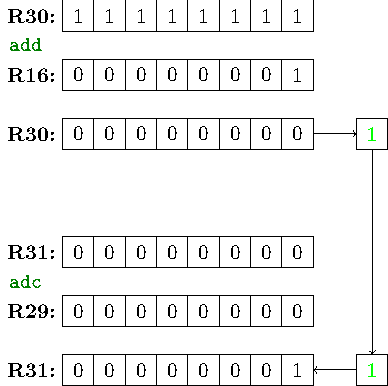
\includegraphics[height = 6cm, keepaspectratio = true]{figures/adc.pdf}
    \caption{Overflow addition using \mintinline{ca65}{adc} in AVR Assembly.} % \label{}
\end{figure}
\subsection{Subtraction}
Subtraction is performed using the same process as binary addition, with the
subtrahend in two's complement form.
In the case of overflows, the carry bit is discarded.
\subsection{Multiplication}
Multiplication is understood as the sum of a set of partial products, similar to the process used in decimal multiplication.
Here each digit of the multiplier is multiplied to the multipicand and each partial product is added to the result.

Given an \(m\)-bit and an \(n\)-bit number, the product is at most \((m+n)\)-bits wide.
\begin{align*}
    13 \times 43 & = 00001101_2 \times 00101011_2                \\
                 & = \begin{aligned}[t]
                          &   & 00001101_2 &  & \times &  & 1_2      \\
                          & + & 00001101_2 &  & \times &  & 10_2     \\
                          & + & 00001101_2 &  & \times &  & 1000_2   \\
                          & + & 00001101_2 &  & \times &  & 100000_2
                     \end{aligned} \\
                 & = \begin{aligned}[t]
                          &   & 00001101_2  \\
                          & + & 00011010_2  \\
                          & + & 01101000_2  \\
                          & + & 110100000_2
                     \end{aligned}                          \\
                 & = 1000101111
\end{align*}
Using AVR assembly, we can use the \keywordinline{mul} instruction to perform multiplication.
\begin{minted}{ca65}
; First number
|\keyword{ldi}| r16, 13
; Second number
|\keyword{ldi}| r17, 43

; Multiply
|\keyword{mul}| r16, r17 ; R1:R0 <- 0b00000010:0b00101111 = 2:47
\end{minted}
The result is stored in the register pair \mintinline{text}{R1:R0}.
\subsection{Division}
Division, square roots and many other functions are very expensive to implement in hardware,
and thus are typically not found in conventional ALUs, but rather
implemented in software.

However, there are other techniques that can be used to implement division in hardware.
By representing the divisor in reciprocal form, we can try to represent the number as
the sum of powers of 2.

For example, the divisor \(6.4\) can be represented as:
\begin{equation*}
    \frac{1}{6.4} = \frac{10}{64} = 10 \times 2^{-6}
\end{equation*}
so that dividing an integer \(n\) by \(6.4\) is approximately equivalent to:
\begin{equation*}
    \frac{n}{6.4} \approx \left( n \times 10 \right) \gg 6
\end{equation*}
When the divisor is not exactly representable as a power of 2 we can use fractional
exponents to represent the divisor, however this requires a floating point
system implementation which is not provided on the AVR\@.
\chapter{Microcontroller Interfacing}
\section{Logic Levels}
\subsection{Discretisation}
The process of discretisation translates a continuous signal into a discrete signal (bits).
As an example, we can translate \textbf{voltage levels} on microcontroller pins into digital \textbf{logic levels}.
\subsection{Logic Levels}
For digital input/output (IO), conventionally:
\begin{itemize}
    \item The voltage level of the positive power supply represents a \textbf{logical 1}, or the \textbf{high state}, and
    \item \qty{0}{V} (ground) represents a \textbf{logical 0}, or the \textbf{low state}.
\end{itemize}
The QUTy is supplied \qty{3.3}{V} so that when a digital output is high,
the voltage present on the corresponding pin will be around \qty{3.3}{V}.
Because voltage is a continuous quantity, we must discretise the full range of voltages into logical levels using \textbf{thresholds}.
\begin{itemize}
    \item A voltage \textbf{above} the input \textbf{high threshold} \(t_H\) is considered \textbf{high}.
    \item A voltage \textbf{below} the input \textbf{low threshold} \(t_L\) is considered \textbf{low}.
\end{itemize}
The interpretation of a voltage between these states is determined by \textbf{hysteresis}.
\subsection{Hysteresis}
Hysteresis refers to the property of a system whose state is \textbf{dependent} on
its \textbf{history}. In electronic circuits, this avoids ambiguity in determining
the state of an input as it switches between voltage levels.
\begin{figure}[H]
    \centering
    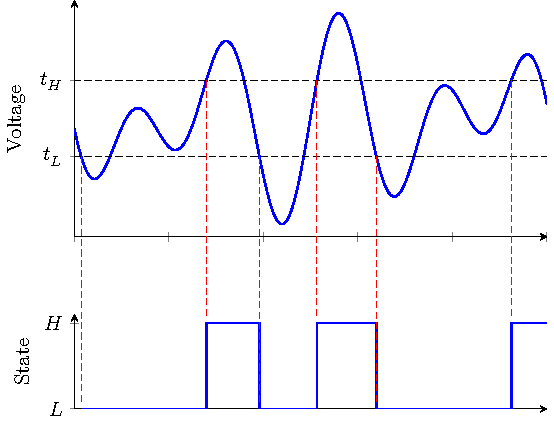
\includegraphics[height = 5cm, keepaspectratio = true]{figures/hysteresis.pdf}
    \caption{Example of hysteresis.} % \label{}
\end{figure}
Given a transition:
\begin{itemize}
    \item If an input is currently in the \textbf{low state}, it has not transitioned to the \textbf{high state} until the voltage crosses the \textbf{high input voltage} threshold.
    \item If an input is currently in the \textbf{high state}, it has not transitioned to the \textbf{low state} until the voltage crosses the \textbf{low input voltage} threshold.
\end{itemize}
It is therefore always preferrable to drive a digital input to an unambiguous voltage level.
\section{Electrical Quantities}
\subsection{Voltage}
\textbf{Voltage} \(v\) is the electrical \textit{potential difference} between two points in a circuit, measured in \textbf{Volts (\unit{V})}.
\begin{itemize}
    \item Voltage is measured across a circuit element, or between two points in a circuit, commonly with respect to a \qty{0}{V} reference (ground).
    \item It represents the \textbf{potential} of the electrical system to do \textbf{work}.
\end{itemize}
\subsection{Current}
\textbf{Current} \(i\) is the \textit{rate of flow of electrical charge} through a circuit, measured in \textbf{Amperes (\unit{A})}.
\begin{itemize}
    \item Current is measured through a circuit element.
\end{itemize}
\subsection{Power}
\textbf{Power} \(p\) is the rate of energy transferred per unit time, measured in \textbf{Watts (\unit{W})}.
Power can be determined through the equation
\begin{equation*}
    p = v i.
\end{equation*}
\subsection{Resistance}
\textbf{Resistance} \(R\) is a property of a material to \textit{resist the flow of current}, measured in \textbf{Ohms (\unit{\ohm})}.
Ohm's law states that the voltage across a component is proportional to the current that flows through it:
\begin{equation*}
    v = i R.
\end{equation*}
Note that not all circuit elements are resistive (or Ohmic), such that they
do not follow Ohm's law, this can be seen in diodes.
\begin{figure}[H]
    \centering
    \begin{subfigure}{0.47\linewidth}
        \centering
        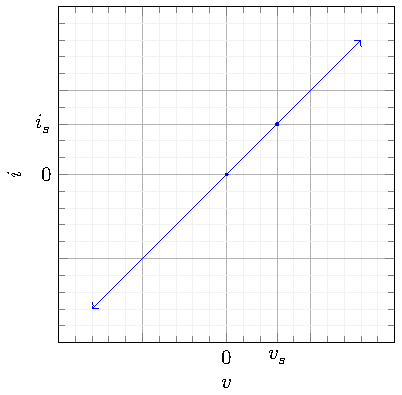
\includegraphics[height=4.5cm]{figures/vi_ohmic.pdf}
        \caption{VI curve for Ohmic components.}
    \end{subfigure}
    \begin{subfigure}{0.47\linewidth}
        \centering
        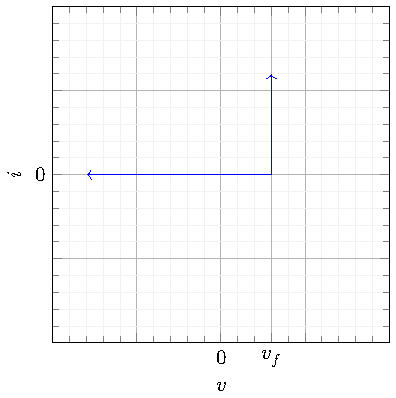
\includegraphics[height=4.5cm]{figures/vi_diode.pdf}
        \caption{VI curve for diodes.}
    \end{subfigure}
    \caption{Voltage-current characteristic curves for various components.}
\end{figure}
Although the wires used to connect a circuit are resistive, we usually assume that they are ideal, that is,
they have zero resistance.
\section{Electrical Components}
\subsection{Resistors}
A \textbf{resistor} is a circuit element that is designed to have a specific resistance \(R\).
\begin{figure}[H]
    \centering
    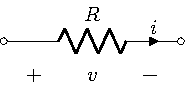
\includegraphics[height = 2.5cm, keepaspectratio = true]{figures/resistor.pdf}
    \caption{Resistor circuit symbol.} % \label{}
\end{figure}
\subsection{Switches}
A \textbf{switch} is used to connect and disconnect different elements in a circuit. It can be \textbf{open}
or \textbf{closed}.
\begin{itemize}
    \item In the \textbf{open} state, the switch \textbf{will not conduct}\footnote{Conductance is a measure of the ability for electric charge to flow in a certain path.} current
    \item In the \textbf{closed} state, the switch \textbf{will conduct} current
\end{itemize}
Switches can take a variety of forms:
\begin{itemize}
    \item \textbf{Poles} --- the number of circuits the switch can control.
    \item \textbf{Throw} --- the number of output connections each pole can connect its input to.
    \item Momentary or toggle action
    \item Different form factors, e.g., push button, slide, toggle, etc.
\end{itemize}
Switches are typically for user input.
\begin{figure}[H]
    \centering
    \begin{subfigure}{0.47\linewidth}
        \centering
        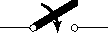
\includegraphics[width=2.5cm]{figures/spst.pdf}
        \caption{Single pole single throw switch.}
    \end{subfigure}
    \begin{subfigure}{0.47\linewidth}
        \centering
        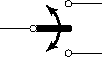
\includegraphics[width=2.5cm]{figures/spdt.pdf}
        \caption{Single pole double throw switch.}
    \end{subfigure}

    \vspace*{5ex}
    \begin{subfigure}{0.47\linewidth}
        \centering
        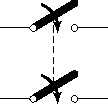
\includegraphics[width=2.5cm]{figures/dpst.pdf}
        \caption{Double pole single throw switch.}
    \end{subfigure}
    \begin{subfigure}{0.47\linewidth}
        \centering
        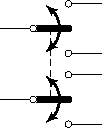
\includegraphics[width=2.5cm]{figures/dpdt.pdf}
        \caption{Double pole double throw switch.}
    \end{subfigure}
    \caption{Various types of switches.}
\end{figure}
\subsection{Diodes}
A \textbf{diode} is a semiconductor device that conducts current in
only one direction: from the \textbf{anode} to the \textbf{cathode}.
\begin{figure}[H]
    \centering
    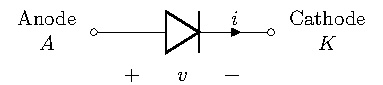
\includegraphics[height = 2cm, keepaspectratio = true]{figures/diode.pdf}
    \caption{Diode symbol.} % \label{}
\end{figure}
Diodes are a non-Ohmic device:
\begin{itemize}
    \item When \textbf{forward biased}, a diode \textbf{does} conduct current, and the anode-cathode voltage
          is equal to the diodes \textbf{forward voltage}.
    \item When \textbf{reverse biased}, a diode \textbf{does not} conduct current, and the cathode-anode voltage
          is equal to the \textbf{applied voltage}.
\end{itemize}
\begin{figure}[H]
    \centering
    \begin{subfigure}{0.47\linewidth}
        \centering
        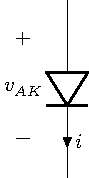
\includegraphics[height=3.5cm]{figures/diode_forward_bias.pdf}
        \caption{Forward biased diode. \\\(v_{AK} = v_f\) and \(i > 0\).}
    \end{subfigure}
    \begin{subfigure}{0.47\linewidth}
        \centering
        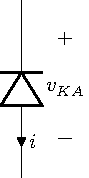
\includegraphics[height=3.5cm]{figures/diode_reverse_bias.pdf}
        \caption{Reverse biased diode. \\\(v_{KA} > 0\) and \(i = 0\).}
    \end{subfigure}
    \caption{Diodes in forward and reverse bias.}
\end{figure}
A diode is only forward biased when the applied anode-cathode voltage \textbf{exceeds} the forward voltage \(v_f\).
A typical forward voltage \(v_f\) for a silicon diode is in the range \qtyrange{0.6}{0.7}{V}, whereas for
Light Emitting Diodes (LEDs), \(v_f\) ranges between \qtyrange{2}{3}{V}.
\subsection{Integrated Circuit}
An \textbf{integrated circuit} (IC) is a set of electronic circuits (typically) implemented on a
single piece of semiconductor material, usually silicon. ICs comprise of hundreds to
many thousands of transistors, resistors and capacitors; all implemented on silicon.
ICs are \textbf{packaged}, and connections to the internal circuitry are exposed via \textbf{pins}.

In general, the specific implementation of the IC is not important, but
rather the \textbf{function of the device} and how it \textbf{interfaces} with the rest of the circuit.
Hence ICs can be treated as a functional \textbf{black box}.
For digital ICs:
\begin{itemize}
    \item \textbf{Input pins} are typically \textbf{high-impedance}, and they appear as an open circuit.
    \item \textbf{Output pins} are typically \textbf{low-impedance}, and will actively drive the voltage
          on a pin and any connected circuitry to a \textbf{high} or \textbf{low} state. They can also
          drive connected loads.
\end{itemize}
\section{Digital Outputs}
Digital output interfaces are designed to be able to drive connected circuitry to one of states,
high, or low, however, the appropriate technique is \textbf{context specific}.
When referring to digital outputs, we will refer to the states of a net. A \textbf{net}
is defined as the common point of connection of multiple circuit components.

In this section we will consider:
\begin{itemize}
    \item What kind of load the output drives
    \item Could more than one device be attempting to actively drive the net
          to a specific logic level?
\end{itemize}
\subsection{Push-Pull Outputs}
A push-pull digital output is the most common form of output used in digital outputs.
The \textbf{output driver} \(A\) \textit{drives} the \textbf{output state} \(Y\) to:
\begin{itemize}
    \item \textbf{HIGH} by connecting the output net to the supply voltage \(+\unit{V}\).
    \item \textbf{LOW} by connecting the output net to the ground voltage GND (\qty{0}{V}).
\end{itemize}
\begin{figure}[H]
    \centering
    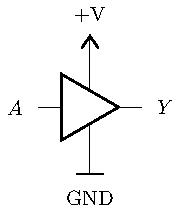
\includegraphics[height = 4cm, keepaspectratio = true]{figures/push_pull.pdf}
    \caption{Push-pull output.} % \label{}
\end{figure}
Hence the output state \(Y\) is determined by the logic level of the output driver \(A\).
\begin{equation*}
    Y = A.
\end{equation*}
\begin{table}[H]
    \centering
    \begin{tabular}{c | c} % chktex 44
        \toprule
        \textbf{\(A\)} & \textbf{\(Y\)} \\
        \midrule
        LOW            & LOW            \\
        HIGH           & HIGH           \\
        \bottomrule
    \end{tabular}
    \caption{Truth table for a push-pull digital output.} % \label{}
\end{table}
The push-pull output \(Y\) can both source and sink current from the connected net.
\subsection{High-Impedance Outputs}
In many instances, a digital output is required to be placed in a high-impedance (HiZ) state.
This is accomplished by using an \textbf{output enable} (OE) signal.
\begin{figure}[H]
    \centering
    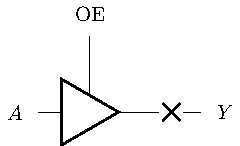
\includegraphics[height = 3cm, keepaspectratio = true]{figures/HiZ.pdf}
    \caption{High-impedance output.} % \label{}
\end{figure}
\begin{itemize}
    \item When the OE signal is \textbf{HIGH}, the output state \(Y\) is determined by the output driver \(A\).
    \item When the OE signal is \textbf{LOW}, the output state \(Y\) is in a \textbf{high-impedance} state.
\end{itemize}
\begin{table}[H]
    \centering
    \begin{tabular}{c c | c} % chktex 44
        \toprule
        \textbf{\(A\)} & \textbf{OE} & \textbf{\(Y\)} \\
        \midrule
        LOW            & LOW         & HiZ            \\
        HIGH           & LOW         & HiZ            \\
        LOW            & HIGH        & LOW            \\
        HIGH           & HIGH        & HIGH           \\
        \bottomrule
    \end{tabular}
    \caption{Truth table for a push-pull digital output.} % \label{}
\end{table}
When the output is in \textbf{HiZ state}:
\begin{itemize}
    \item The output is an effective \textbf{open circuit}, meaning it has \textbf{no effect} on the rest of the circuit.
    \item The voltage on the output net is determined by the \textbf{other circuitry} connected to the net.
\end{itemize}
HiZ outputs are typically used when multiple need to signal over the same wire(s).
\subsection{Pull-up and Pull-down Resistors}
When \textbf{no devices} are actively driving a net (e.g., all connected outputs are in the HiZ state),
the state of the net is not well-defined. Hence we can use a \textbf{pull-up} or \textbf{pull-down} resistor
to ensure that the state of the pin is always \textbf{well-defined}.
\pagebreak
\begin{multicols}{2}
    \begin{figure}[H]
        \centering
        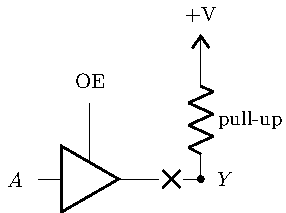
\includegraphics[height = 4cm, keepaspectratio = true]{figures/pullup_resistor.pdf}
        \caption{Pull-up resistor.} % \label{}
    \end{figure}
    \begin{figure}[H]
        \centering
        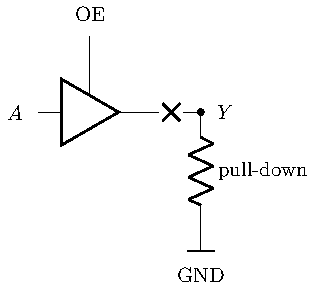
\includegraphics[height = 4cm, keepaspectratio = true]{figures/pulldown_resistor.pdf}
        \caption{Pull-down resistor.} % \label{}
    \end{figure}
\end{multicols}
\begin{itemize}
    \item When \textbf{no circuitry} is actively driving the net, the resistor will passively pull the voltage to either the voltage supply, or ground.
    \item When \textbf{another device} actively drives the net, the active device defines the voltage of the net. Hence the current from the resistor is simply sourced
          or sunk by the \textbf{active device}.
\end{itemize}
The resistors used as pull-up and pull-down resistors are typically in the \unit{k\ohm} range.
\subsection{Open-Drain Outputs}
Multiple push-pull outputs should never be connected to the same net
as when one output is driven HIGH and another is driven LOW,
an effective short circuit is created and one or more devices may be damaged.
While push-pull outputs with an output enable may be used,
the timing must be carefully managed.

Hence a more robust solution is to use open-drain outputs.
\begin{figure}[H]
    \centering
    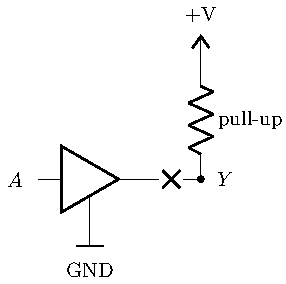
\includegraphics[height = 4cm, keepaspectratio = true]{figures/open_drain.pdf}
    \caption{Open-drain output.} % \label{}
\end{figure}
An open-drain output is either:
\begin{itemize}
    \item In the \textbf{high-impedance} state, where the pull-up resistor is used to pull the net to the \textbf{high state} when the net is \textbf{not driven low}.
    \item \textbf{Connected to ground}, when the net is \textbf{driven low}.
\end{itemize}
\section{Microcontroller Pins}
Microcontrollers are interfaced via their exposed pins.
These pins are the only means to access inputs and outputs, and
they are used to interface with other electronic circuits in order to achieve a required functionality.
Pins can be used for:
\begin{itemize}
    \item General purpose input and output (GPIO) --- pin represents a digital state
    \item Peripheral functions
    \item Other functions (power supply, reset input, clock input, etc.)
\end{itemize}
Pins are typically organised into groups of related IO banks,
referred to as \textbf{ports} on the AVR microcontroller.
These ports and pins are assigned an alphanumeric identifier, (e.g., PB7 for pin 7 on port B).
\begin{figure}[H]
    \centering
    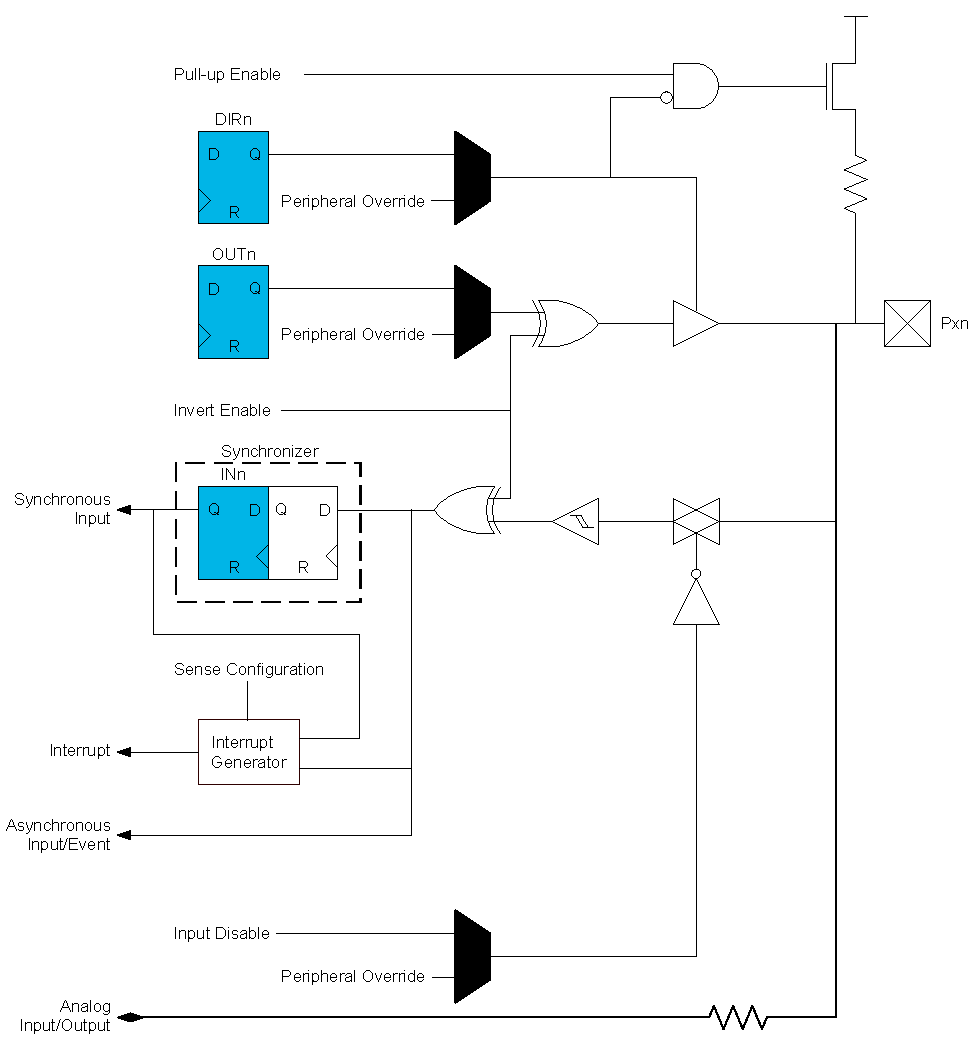
\includegraphics[height = 10cm, keepaspectratio = true]{figures/PORT_block_diagram.pdf}
    \caption{ATtiny1626 PORT block diagram.} % \label{}
\end{figure}
To summarise this diagram:
\begin{itemize}
    \item The data direction register (DIR) controls the push-pull output enable.
    \item The output driver register (OUT) drives the output state.
    \item The input register (IN) reads the output state.
    \item The internal pull-up register enabled through software.
    \item The physical voltage on the pin can be routed to an analogue to digital converter (ADC)
    \item Other peripheral functions can override port pin configurations and the output state.
\end{itemize}
\subsection{Configuring an Output in Assembly}
\begin{enumerate}
    \item Place the port pin in a \textbf{safe initial state}
          by writing to the OUT register (HIGH or LOW depending on the context).
    \item Configure the port pin as an output by \textbf{setting} the corresponding bits in the DIR register.
    \item Set the desired pin state by writing to the OUT register.
\end{enumerate}
\begin{minted}{ca65}
; Load macros for easy access to port data space addresses.
#include <avr/io.h>

; Bitmask for pin 5
|\keyword{ldi}| r16, PIN5_bm

; Set initial safe state
|\keyword{sts}| PORTB_OUTCLR, r16 ; LOW if active HIGH
|\keyword{sts}| PORTB_OUTSET, r16 ; HIGH if active LOW

; Enable output
|\keyword{sts}| PORTB_DIRSET, r16 ; Enable output on PB5

; Set output state to desired value
|\keyword{sts}| PORTB_OUTSET, r16 ; Set state of PB5 to HIGH
\end{minted}
\subsection{Configuring an Input in Assembly}
\begin{enumerate}
    \item If required, enable the internal pull-up resistor by \textbf{setting}
          the PULLUPEN bit in the \linebreak corresponding PINnCTRL register.
    \item Read the IN register to get the current state of the pin.
    \item Isolate the relevant pin using the AND operator.
\end{enumerate}
\begin{minted}{ca65}
#include <avr/io.h>

|\keyword{ldi}| r16, PIN5_bm

; Enable internal pull-up resistor if required
|\keyword{sts}| PORTB_PIN5CTRL, r16

; Read output state from data space
|\keyword{lds}| r17, PORTA_IN
; Read output state using virtual PORT
|\keyword{in}| r17, VPORTA_IN

; Isolate desired pin
|\keyword{andi}| r17, r16
\end{minted}
\subsection{Peripheral Multiplexing}
Pins can be used to connect internal peripheral functions
to external devices.
As microcontrollers have more peripheral functions than available pins,
peripheral functions are typically multiplexed onto pins.
\begin{definition}[Multiplexing]
    Multiplexing is a method by which \textbf{multiple peripheral} \linebreak \textbf{functions}
    are mapped to the \textbf{same pin}.
    In this scenario, only one function can be enabled at a time, and the pin
    cannot be used for GPIO\@.
\end{definition}
\begin{itemize}
    \item Peripheral functions can be mapped to different \textbf{sets of pins} to provide
          flexibility and to avoid clashes when multiple peripherals are used in
          an application.
    \item When enabled, peripheral functions \textbf{override} standard port functions.
    \item The \textbf{Port Multiplexer} (PORTMUX) is used to select which
          \textbf{pin set} should be used by a peripheral.
    \item Certain peripherals can have their inputs/outputs mapped to different
          \textbf{sets of pins} through the PORTMUX\@.
\end{itemize}
Note that we cannot re-map a single peripheral function to another pin, but must consider the entire set.
\section{Interfacing to Simple IO}
\subsection{Driving LEDs}
The \textbf{brightness} of an LED is proportional to the \textbf{current}
passing through it. As LEDs are non-Ohmic, we cannot drive them directly
with a voltage as this would result in an uncontrolled flow of current that
may damage the LED or driver.

Instead, LEDs are paired with a \textbf{series resistor} to limit the flow of current.
The appropriate current is dependent on the specific LED that is used
and the capability of the driver device (microcontroller).
A typical indictor LED requires a current of \qtyrange{1}{2}{m.A}.
\subsection{Interfacing to LEDs}
An LED can be driven in two different configurations from a microcontroller pin:
\begin{itemize}
    \item \textbf{active high}; in which case the LED is \textbf{lit} when the pin is \textbf{HIGH}.
    \item \textbf{active low}; in which case the LED is \textbf{lit} when the pin is \textbf{LOW}.
\end{itemize}
Both of these configurations have their benefits, and the best configuration depends entirely on the context.
\begin{multicols}{2}
    \begin{figure}[H]
        \centering
        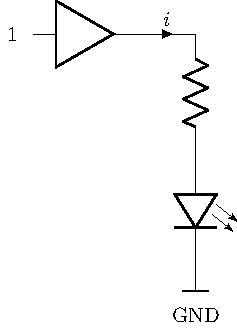
\includegraphics[height = 4cm, keepaspectratio = true]{figures/active_high_LED.pdf}
        \caption{Active high configuration.} % \label{}
    \end{figure}
    \begin{figure}[H]
        \centering
        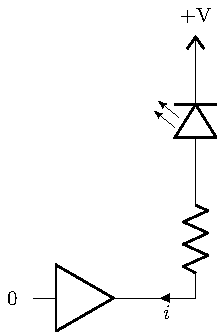
\includegraphics[height = 4cm, keepaspectratio = true]{figures/active_low_LED.pdf}
        \caption{Active low configuration.} % \label{}
    \end{figure}
\end{multicols}
On the QUTy, the LED display is driven in the \textbf{active low} configuration.
This has a number of advantages:
\begin{itemize}
    \item If the internal pull-up resistors are mistakenly enabled, no current will
          flow into the LEDs.
    \item The microcontroller pins can sink higher currents than they can source,
          allowing us to drive the display to a higher brightness.
    \item The display used on the QUTy has a common anode configuration, hence we must use an
          active low configuration to drive the display segments independently.
\end{itemize}
An LED is an example of a simple \textbf{digital output}, as we can map \textbf{logical states}
to \textbf{LED states} (lit or unlit) for a digital output.
\subsection{Switches as Digital Inputs}
The state of a switch can be used to \textbf{set} the state of a pin.
As the switch has two states (open or closed), these can be mapped directly to
\textbf{logical states}.
This can be done by connecting the switch between the pin and voltage source
representing one of the logic levels (ground or a positive supply).
\pagebreak
\begin{multicols}{2}
    \begin{figure}[H]
        \centering
        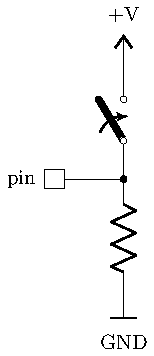
\includegraphics[height = 5cm, keepaspectratio = true]{figures/active_high_switch.pdf}
        \caption{Active high configuration.} % \label{}
    \end{figure}
    \begin{figure}[H]
        \centering
        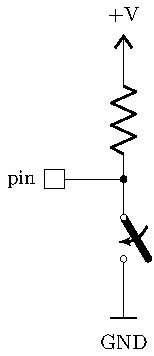
\includegraphics[height = 5cm, keepaspectratio = true]{figures/active_low_switch.pdf}
        \caption{Active low configuration.} % \label{}
    \end{figure}
\end{multicols}
\begin{itemize}
    \item When the switch is \textbf{open}, the pull-up/pull-down resistor is used to define the state of the switch.
    \item When the switch is \textbf{closed}, the state of the pin is defined by the voltage connected to via the switch.
\end{itemize}
\subsection{Interfacing to Switches}
As with LEDs, we can interface switches to microcontroller pins in two different configurations:
\begin{itemize}
    \item \textbf{active high}; in which case the pin is \textbf{HIGH} when the switch is \textbf{closed}.
    \item \textbf{active low}; in which case the pin is \textbf{LOW} when the switch is \textbf{closed}.
\end{itemize}
An \textbf{active low} configuration is usually preferred as:
\begin{itemize}
    \item it allows for the utilisation of an \textbf{internal pull-up resistor} that is commonly
          implemented in microcontrollers.
    \item It eliminates the risk of unsafe voltages being applied to the pin from the power supply in an active high configuration.
    \item It is easier to access a ground reference on a circuit board.
\end{itemize}
\subsection{Interfacing to Integrated Circuits}
For digital ICs,
\begin{itemize}
    \item \textbf{Inputs} are typically \textbf{high impedance}
    \item \textbf{Outputs} are typically \textbf{push-pull}
\end{itemize}
This generally means that we can interface an IC by connecting its pins directly to the pins of a microcontroller.
\begin{itemize}
    \item For \textbf{IC inputs}, the microcontroller pin is configured as an \textbf{output},
          and the \textbf{microcontroller sets} the logic level of the net.
    \item For \textbf{IC outputs}, the microcontroller pin is configured as an \textbf{input},
          and the \textbf{IC sets} the logic level of the net.
\end{itemize}
As microcontroller pins are typically configured as \textbf{inputs on reset}, a
pull-up/pull-down resistor may be required if it is important for an IC input to
have a \textbf{known state} prior to the configuration of the relevant microcontroller pins as outputs.
\part{Assembly Programming}
\begin{definition}[Word]
    A word refers to a value that is two bytes in size (16-bit).
\end{definition}
\section{Registers}
A register refers to a memory location that is 1 byte in size (8-bit).
The ATtiny1626 has 32 registers of which \mintinline{ca65}{r16} to \mintinline{ca65}{r31} can be loaded with an immediate value (\numrange{0}{255}) using \keywordinline{ldi}.
\begin{minted}{ca65}
|\keyword{ldi}| r16, 17 ; Load the value 17 into r16
\end{minted}
Values are commonly loaded into registers as many other operations can be performed on them.
\section{Flow Control}
Instructions on the AVR Core increment the PC by 1 or 2 (depending on whether the OPCODE is 1 or 2 words) when they are executed so that any successive
instructions are executed after the first. To divert execution to a different location, we can utilise
\textbf{change of flow} instructions.

The \mintinline{ca65}{jmp} (jump) instruction is used to simply jump to a different location in the program.
This instruction is capable of jumping to an address withtin the entire 4M (words) program memory, however,
this is highly excessive for the ATtiny1626.
\section{Labels}
Most change of flow instructions take an \textbf{address} in program memory as a parameter.
Hence to make this process easier, we can use labels to refer to locations in program memory (and also RAM).
\begin{minted}{ca65}
jmp new_location ; Jump to the label |\textbf{new\_location}|.
|\keyword{ldi}| r16, 1 ; This instruction is skipped

new_location: ; Label
    |\keyword{push}| r16
\end{minted}
When a label appears in source code, the assembler replaces references to it with the address of the
directive/instruction immediately following that label. Labels work for both \textbf{absolute} and \textbf{relative}
addresses and the assembler will automatically adjust the address to the correct type.

Additionally, labels can also be used as parameters to other immediate instructions if we store the high and low
bytes in registers and wish to reference the location in an indirect jumping instruction.
\section{Absolute and Relative Addresses}
\mintinline{ca65}{jmp} is a 32-bit instruction, which uses 22 bits to specify an address between \mintinline{ca65}{0x000000} % chktex 29
and \mintinline{ca65}{0x3FFFFF}, or \(2^{23} - 1\) bits of memory (\qty{8}{MB}). As mentioned earlier, this is much larger % chktex 29
than what the 16-bit PC can address on the ATtiny1626 (\qty{64}{KB}).

As we will only need to jump within \qty{64}{KB} of memory, it is inefficient to use the \mintinline{ca65}{jmp} instruction as it
requires 3 CPU cycles to execute. Therefore, many AVR change of flow instructions take a value that is
\textbf{added} onto the current PC to calculate the destination address, allowing them to fit within 16 bits.
The \keywordinline{rjmp} (relative jump) instruction is therefore more suitable as it only requires 2
CPU cycles.

Note the assembler throw an error if the address is not within the range of the PC\@.
\section{Branching}
A branching instruction jumps to a different location based on a condition, i.e., user input, internal state, or other external factors.
Many change of flow instructions are conditional, and will alter the PC differently based on register value(s) or flags.
In AVR there are two main categories of branching instructions:
\begin{itemize}
    \item Branch instructions
    \item Skip instructions
\end{itemize}
\subsection{Branch Instructions}
Branch instructions use the following logic:
\begin{enumerate}
    \item Check if the specified flag in SREG is cleared/set
    \item If true, jump to the specified address (\(\mathrm{PC} \leftarrow \mathrm{PC} + k + 1\))
    \item Otherwise, proceed to the next instruction as normal (\(\mathrm{PC} \leftarrow \mathrm{PC} + 1\))
\end{enumerate}
Although there are are 20 branch instructions listed in the instruction set summary, the following two form the basis of all branching instructions:
\begin{itemize}
    \item \keywordinline{brbc} (branch if bit in SREG is cleared)
    \item \keywordinline{brbs} (branch if bit in SREG is set)
\end{itemize}
All other branching instructions are specific cases of the above instructions, that are provided to make programming in Assembly easier.
As these instructions check the bits in the SREG, they are usually preceded by an ALU operation such as \keywordinline{cp} or \keywordinline{cpi} to trigger the required flags.

As only 7 bits are allocated to the destination in the OPCODE, branch instructions jump shorter distances than relative jumps.
\subsection{Compare Instructions}
Both the \keywordinline{cp} and \keywordinline{cpi} instructions are used to compare the values in one or two registers.
The ALU performs a subtraction operation whose result is used to update the SREG\@. Note that the result is not stored or used in any way.
\begin{itemize}
    \item \mintinline{ca65}{|\keyword{cp}| Rd, Rr} performs \mintinline{ca65}{Rd} \(-\) \mintinline{ca65}{Rr}
    \item \mintinline{ca65}{|\keyword{cpi}| Rd, K} performs \mintinline{ca65}{Rd} \(-\) \mintinline{ca65}{K}
\end{itemize}
\begin{minted}{ca65}
|\keyword{ldi}| r16, 0
|\keyword{ldi}| r19, 10
|\keyword{cp}| r16, r19 ; Compare values in registers r16 and r19
|\keyword{brge}| new_location ; Branch if r16 greater than or equal to r19

new_location:
\end{minted}
Note that many instructions are able to set the Z flag, which is used to indicate if the result of the operation is zero.
In these cases, the compare instruction may be redundant.
\subsection{Skip Instructions}
The skip instructions are less flexible then branch instructions, but can sometimes require less space or fewer cycles.
Skip instructions skip the next instruction if the condition is true.

In this example we will skip the line which increments register 16.
\begin{minted}{ca65}
|\keyword{cpse}| r16, r17 ; Skips next instruction if r16 == r17
inc r16 ; This is skipped
\end{minted}
Same example which uses a branch instruction:
\begin{minted}{ca65}
|\keyword{cp}| r16, r17
|\keyword{breq}| new_location ; Skips to new_location if r16 == r17
inc r16 ; This is skipped

new_location: ; PC is now here
\end{minted}
Note that the number of cycles for a skip instruction depends on the size of the instruction being skipped.
The \keywordinline{sbrc} and \keywordinline{sbrs} instructions are used to skip the next instruction if the specified bit a register is cleared/set.
\begin{minted}{ca65}
|\keyword{ldi}| r16, 0b00101110

|\keyword{sbrc}| r16, 0 ; Skips next instruction if bit 0 of r16 is cleared
inc r16 ; This is skipped
\end{minted}
Comparing with branch instructions
\begin{minted}{ca65}
|\keyword{ldi}| r16, 0b00101110
|\keyword{andi}| r16, 0b00000001 ; Isolate bit 0
|\keyword{breq}| new_location ; Skips next instruction if r16 == 0
inc r16 ; This is skipped

new_location: ; PC is now here
\end{minted}
The \keywordinline{sbis} and \keywordinline{sbic} instructions are used to skip the next instruction if the specified bit an I/O register is set/cleared.
For example, if we wish to toggle the decimal point LED (DISP DP) on the QUTy (PORT B pin 5) when the first button (BUTTON0) was pressed (PORT A pin 4),
\begin{minted}{ca65}
|\keyword{ldi}| r16, PIN5_bm ; Bitmask of pin 5
|\keyword{sbis}| VPORTA_IN, 0b00010000 ; Skip next instruction if pin 4 of PORT A is set
|\keyword{sts}| PORTB_OUTTGL, r16 ; Toggle the output driver of pin 5 on PORT B
\end{minted}
Using branch instructions:
\begin{minted}{ca65}
|\keyword{in}| r17, VPORTA_IN ; Read the input register of PORT A
|\keyword{andi}| r17, 0b00010000 ; Isolate pin 4

|\keyword{brne}| new_location ; Skip instructions if r17 != 0

|\keyword{ldi}| r16, PIN5_bm ; Bitmask of pin 5
|\keyword{sts}| PORTB_OUTTGL, r16 ; Toggle the output driver of pin 5 on PORT B

new_location:
\end{minted}
\section{Loops}
By jumping to an earlier address, we can loop over a block of instructions.
\begin{minted}{ca65}
infinite_loop:
    ; Code to repeat
    |\keyword{rjmp}| infinite_loop
\end{minted}
Loops can also be finite, in which case the loop will terminate when a counter reaches zero.
\begin{minted}{ca65}
|\keyword{ldi}| r16, 10 ; Set counter to 10
loop:
    dec r16 ; Decrement counter
    |\keyword{brne}| loop ; Branch if counter != 0
\end{minted}
Loops can also be used to repeat until some external event occurs.
\begin{minted}{ca65}
main_loop:
    |\keyword{in}| r17, VPORTA_IN ; Read the input register of PORT A
    |\keyword{andi}| r17, 0b00010000 ; Isolate pin 4

    |\keyword{brne}| main_loop ; Branch if counter != 0
    |\keyword{rjmp}| button_pressed

button_pressed:
    ; Execute instructions
    |\keyword{rjmp}| main_loop ; Return to main loop
\end{minted}
\section{Delays}
Loops can be utilised to delay the execution of instructions. These instructions do
not execute any useful code. This is useful for when we wish to wait for an external event to occur.\footnote{Note that this type of loop is not recommended for time-sharing systems, such as a personal computer, as the lost CPU cycles cannot be used by other programs. In these cases, clock interrupts are preferred. However, on a device such as the ATtiny1626, delay loops can be utilised to precisely insert delays in a program.}

To create a precisely timed delay, we must take the following values into account.
\begin{itemize}
    \item The clock speed --- frequency of the clocks oscillations (default: \qty{20}{MHz} --- configurable in CLKCTLR\_MCLKCTRLA)
    \item The prescaler --- reduces the frequency of the CPU clock through division by a specific amount; 12 different settings from 1x to 64x (default: 6 --- configurable in CLKCTLR\_MCLKCTRLA)
\end{itemize}
The clock oscillates at its effective clock speed:
\begin{equation*}
    \text{effective clock speed} = \text{clock speed} \times \frac{1}{\text{prescaler}}
\end{equation*}
The default prescaler is 6, so the effective clock speed is \qty{3.33}{MHz} by default.
Note that the effective clock speed can therefore range between:
\begin{itemize}
    \item Effective maximum clock frequency: \qty{20}{MHz} (\qty{20}{MHz} clock \& prescaler 1)\footnote{As the QUTy is supplied with \qty{3.3}{V}, it is not safe to go above \qty{10}{MHz}.}
    \item Effective minimum clock frequency: \qty{512}{Hz} (\qty{32.768}{kHz} clock \& prescaler 64)
\end{itemize}
Therefore to create a delay, we must first determine the required number of CPU cycles in the body of the loop
and iterate until the number of CPU cycles reaches the required amount.

The following examples utilise counters of various sizes to create delays.
Note that \(n\) represents the number of iterations.
\begin{minted}{ca65}
delay_1:
|\keyword{ldi}| r16, x ; 1 CPU cycle
|\keyword{ldi}| r17, 1 ; 1 CPU cycle ; Incrementor

loop:
    add r16, r17 ; 1 CPU cycle
    |\keyword{brcc}| loop ; 2 CPU cycles (1 CPU cycle when condition is false)
\end{minted}
The register \mintinline{ca65}{r16} has the following relationship:
\begin{equation*}
x = \left( 2^8 - 1 \right) - n \iff n = \left( 2^8 - 1 \right) - x
\end{equation*}
with
\begin{align*}
    \text{total cycles} & = 1 + 1 + \left( n + 1 \right) + 2 n + 1 \\
                        & = 3 n + 4
\end{align*}
for a maximum delay of \qty{230.7}{\micro s} (\(\left( 3 \times \left( 2^8 - 1 \right) + 4 \right) T\))\footnote{\(T\) is the period of one CPU cycle (using the default clock configuration): \(T = \frac{1}{\qty{20}{MHz} / 6} = \qty{300}{ns}\).}.
To create larger delays, we can use multiple registers:
\begin{minted}{ca65}
delay_2:
    |\keyword{ldi}| r24, x ; 1 CPU cycle
    |\keyword{ldi}| r25, y ; 1 CPU cycle

    loop:
        |\keyword{adiw}| r24, 1 ; 2 CPU cycles
        |\keyword{brcc}| loop ; 2 CPU cycles (1 CPU cycle when condition is false)
\end{minted}
The register pair \(\left( y:x \right)\) has the following relationship:
\begin{align*}
    \left( y:x \right) = \left( 2^{16} - 1 \right) - n \iff n = \left( 2^{16} - 1 \right) - \left( y:x \right)
\end{align*}
with
\begin{align*}
    \text{total cycles} & = 1 + 1 + 2 \left( n + 1 \right) + 2 n + 1 \\
                        & = 4n + 5
\end{align*}
for a maximum delay of \qty{78.644}{ms} (\(\left(4 \times \left( 2^{16} - 1 \right) + 5 \right) T\)).
With three registers,
\begin{minted}{ca65}
delay_3:
    |\keyword{ldi}| r24, x ; 1 CPU cycle
    |\keyword{ldi}| r25, y ; 1 CPU cycle
    |\keyword{ldi}| r26, z ; 1 CPU cycle

    loop:
        |\keyword{adiw}| r24, 1 ; 2 CPU cycles
        |\keyword{adc}| r26, r0 ; 1 CPU cycle (r0 represents a register with value 0)
        |\keyword{brcc}| loop ; 2 CPU cycles (1 CPU cycle when condition is false)
\end{minted}
The register triplet \(\left( z:y:x \right)\) is determined through:
\begin{align*}
    \left( z:y:x \right) = \left( 2^{24} - 1 \right) - n \iff n = \left( 2^{24} - 1 \right) - \left( z:y:x \right)
\end{align*}
with
\begin{align*}
    \text{total cycles} & = 1 + 1 + 1 + 2 \left( n + 1 \right) + \left( n + 1 \right) + 2 n + 1 \\
                        & = 5n + 7
\end{align*}
for a maximum delay of \qty{25.166}{s} (\(\left(5 \times \left( 2^{24} - 1 \right) + 7 \right) T\)).
This approach can be extended to create delays of any length.

If needed, we can also include the \mintinline{ca65}{nop} (no operation) instruction which requires 1 CPU cycle and does nothing.
In addition to this, we can also utilise nested loops, however the timing is more complex to determine.
\section{Memory and IO}
On the AVR Core, as both I/O and SRAM are accessed through the data space, they can be
directly accessed using instructions that read/write to memory. This approach is known as memory-mapped I/O (MMIO)
and it significantly reduces chip complexity.

In contrast to modern CPU architectures, such as x86, in the AVR architecture,
programs are located in a separate address space (although the memory is still accessible through the data space).
\begin{figure}[H]
    \centering
    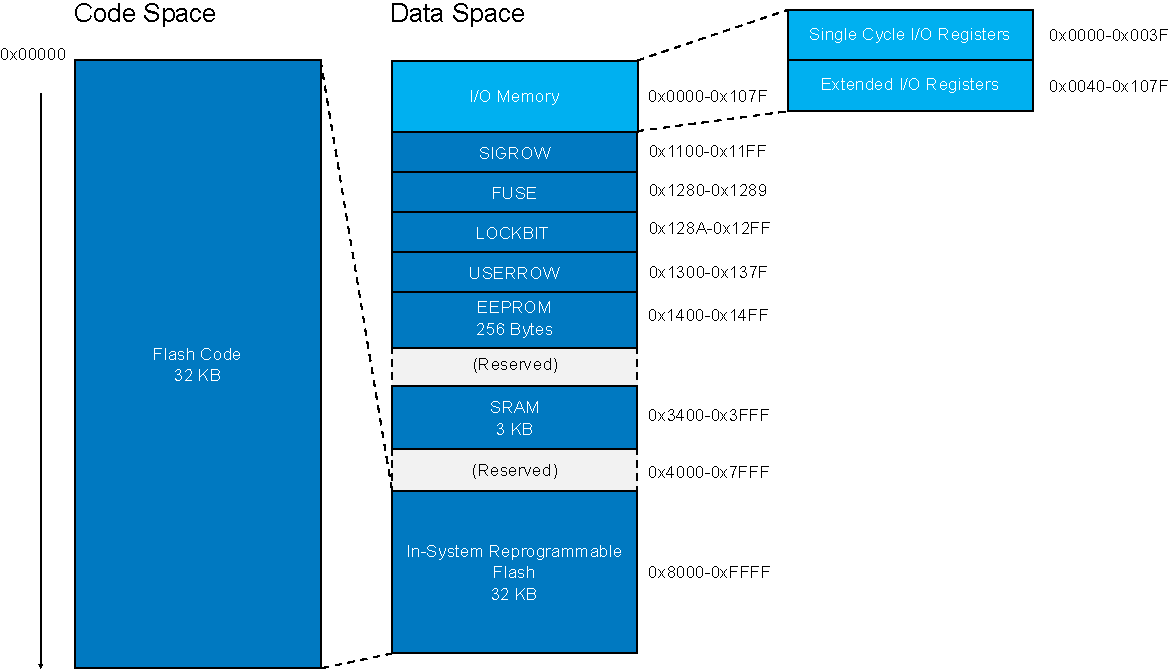
\includegraphics[height = 8cm, keepaspectratio = true]{figures/memory_map.pdf}
    \caption{ATtiny1626 memory map.} % \label{}
\end{figure}
The following instructions may be used to access memory from the data space:
\begin{itemize}
    \item \keywordinline{lds} (load direct from data space to register)
    \item \keywordinline{sts} (store direct from register to data space)
    \item \keywordinline{ld} (load indirect from data space to register)
    \item \keywordinline{st} (store indirect from register to data space)
    \item \keywordinline{push}/\keywordinline{pop} (stack operations in SRAM --- starting at \mintinline{ca65}{0x3800}) % chktex 29
    \item \keywordinline{in}/\keywordinline{out} (single cycle I/O register operations)
    \item \keywordinline{sbi}/\keywordinline{cbi} (set/clear bit in I/O register)
\end{itemize}
Note that the \keywordinline{in}/\keywordinline{out} instructions can
only access the low 64 bytes of the I/O register space and the \keywordinline{sbi}/\keywordinline{cbi}
instructions can only access the low 32 bytes of the I/O register space.

As the name suggests, these instructions only require a single CPU cycle and hence
several addresses such as VPORT\{A, B, C\} (virtual ports) are mapped to this location,
for fast access.
\subsection{Load/Store Indirect}
While the \keywordinline{lds}/\keywordinline{sts} instructions can be used to access addresses
of bytes, they are generally not suitable for accessing data structures such as arrays.
Instead, we can use the \keywordinline{ld}/\keywordinline{st} instructions to
take advantage of their 16-bit pointer registers, which support some pointer arithmetic.
\begin{itemize}
    \item \mintinline{ca65}{r26} \(\to\) \keywordinline{XL} (\keywordinline{X}-register low byte)
    \item \mintinline{ca65}{r27} \(\to\) \keywordinline{XH} (\keywordinline{X}-register high byte)
    \item \mintinline{ca65}{r28} \(\to\) \keywordinline{YL} (\keywordinline{Y}-register low byte)
    \item \mintinline{ca65}{r29} \(\to\) \keywordinline{YH} (\keywordinline{Y}-register high byte)
    \item \mintinline{ca65}{r30} \(\to\) \keywordinline{ZL} (\keywordinline{Z}-register low byte)
    \item \mintinline{ca65}{r31} \(\to\) \keywordinline{ZH} (\keywordinline{Z}-register high byte)
\end{itemize}
For example, if we wanted to access a byte in RAM, we can do the following:
\begin{minted}{ca65}
|\keyword{ldi}| XL, lo8(RAMSTART) ; Store address of RAM in X
|\keyword{ldi}| XH, hi8(RAMSTART)

|\keyword{ld}| r16, X ; Load byte from X to r16
; The byte in X is now in r16

|\keyword{ldi}| r17, 24
|\keyword{st}| X, r17 ; Store byte from r16 to X
; The byte in X (and hence at RAMSTART) is now 24
\end{minted}
These pointer registers also support post-increment and pre-decrement operations:
\begin{itemize}
    \item \mintinline{ca65}{X+} (post-increment pointer address)
    \item \mintinline{ca65}{-X} (pre-decrement pointer address)
\end{itemize}
\begin{minted}{ca65}
|\keyword{ld}| r16, X+ ; Load byte from X to r16, then X <- X + 1
|\keyword{st}| X+, r16 ; Store byte from r16 to X, then X <- X + 1

|\keyword{ld}| r16, -X ; X <- X - 1, then load byte from X to r16
|\keyword{st}| -X, r16 ; X <- X - 1, then store byte from r16 to X
\end{minted}
This operation can be used to copy bytes from one location to another:
\begin{minted}{ca65}
; Copy 10 bytes from RAM to RAM+10
|\keyword{ldi}| XL, lo8(RAMSTART)
|\keyword{ldi}| XH, hi8(RAMSTART)

|\keyword{ldi}| YL, lo8(RAMSTART+10)
|\keyword{ldi}| YH, hi8(RAMSTART+10)

|\keyword{ldi}| r16, 10 ; Loop 10 times
loop:
    |\keyword{ld}| r0, X+ ; Load byte from X to r0, then X <- X + 1
    |\keyword{st}| Y+, r0 ; Store byte from r0 to Y, then Y <- Y + 1
    dec r16
    |\keyword{brne}| loop
\end{minted}
\subsection{Load/Store Indirect with Displacement}
In addition to the \keywordinline{ld}/\keywordinline{st} instructions, the \keywordinline{ldd}/\keywordinline{std}
instructions are a special form that allow us to load/store from/to the address of the pointer register
\textbf{plus} \(q = \left\{ \numrange{0}{63} \right\}\).
\begin{minted}{ca65}
|\keyword{ldi}| YL, lo8(RAMSTART)
|\keyword{ldi}| YH, hi8(RAMSTART)

|\keyword{ldd}| r0, Y+20 ; Load byte from Y+20 to r0
|\keyword{std}| Y+21, r0 ; Store byte from r1 to Y+21
; Note Y still points to RAMSTART
\end{minted}
Note this form is only available for \keywordinline{Y}, and \keywordinline{Z}.
\section{Stack}
The stack is a last-in first-out (LIFO) data structure in SRAM\@.
It is accessed through a register called the stack pointer (SP),
which is not part of the register file like SREG\@.

Upon reset, SP is set to the last available address in SRAM (\mintinline{ca65}{0x3FFF}), % chktex 29
and can be modified through \keywordinline{push}/\keywordinline{pop} and other methods that are generally not recommended.
\begin{itemize}
    \item \keywordinline{push} stores a register to SP then decrements SP (\(\mathrm{SP} \leftarrow \mathrm{SP} - 1\))
    \item \keywordinline{pop} increments SP (\(\mathrm{SP} \leftarrow \mathrm{SP} + 1\)) then loads to a register from SP
\end{itemize}
If a particular register is required without modifying other code, we can temporarily
store the value of that register on the stack, and pop it back when we are done:
\begin{minted}{ca65}
|\keyword{push}| ZL ; Temporarily store Z on the stack
|\keyword{push}| ZH
; Z may be used for another purpose
|\keyword{pop}| ZH ; Restore Z from the stack in reverse order
|\keyword{pop}| ZL
\end{minted}
\section{Procedures}
Procedures allow us to write modular, reusable code which makes them powerful when working on
complex projects. Although they are usually associated with high level languages as
methods, or functions, they are also available in assembly.

Procedures begin with a label, and end with the \mintinline{ca65}{ret} keyword.
They must be \textbf{called} using the \keywordinline{call}/\keywordinline{rcall} instructions.
\begin{minted}{ca65}
procedure:
    ; Procedure body
    |\keyword{ret}| ; Return to caller
\end{minted}
\subsection{Saving Context}
To ensure that procedures are maximally flexible and place no constraints on the caller,
we must always restore any modified registers before returning to the caller. The same is
true for the SREG\@.
\begin{minted}{ca65}
|\keyword{rjmp}| main_loop

procedure:
    |\keyword{push}| r16 ; Save r16 on the stack
    ; Code that possibly modifies r16
    |\keyword{pop}| r16 ; Restore r16 from the stack
    |\keyword{ret}|

main_loop:
    |\keyword{ldi}| r16, 10
    |\keyword{rcall}| procedure ; Call procedure
    |\keyword{push}| r16 ; r16 should still be 10
\end{minted}
\subsection{Parameters and Return Values}
Parameters can be passed using registers or the stack depending on the size of
the inputs.
\begin{minted}{ca65}
|\keyword{rjmp}| main_loop

; Calculate the average of two numbers
; Inputs:
;     r16: first number
;     r17: second number
; Outputs:
;     r16: average
average:
    |\keyword{push}| r0 ; Save r0
    |\keyword{in}| r0, CPU_SREG ; Save SREG
    |\keyword{push}| r0

    ; Calculate average
    |\keyword{add}| r16, r17
    ror r16

    |\keyword{pop}| r0 ; Restore SREG
    |\keyword{out}| CPU_SREG, r0
    |\keyword{pop}| r0 ; Restore r0
    |\keyword{ret}|

main_loop:
    ; Arguments
    |\keyword{ldi}| r16, 100
    |\keyword{ldi}| r17, 200
    |\keyword{rcall}| average
\end{minted}
Using the stack:
\begin{minted}{ca65}
|\keyword{rjmp}| main_loop

; Calculate the average of two numbers
; Inputs:
;     top two values on stack
; Outputs:
;     r16: average
average:
    |\keyword{push}| ZL ; Save Z
    |\keyword{push}| ZH
    |\keyword{in}| ZL, CPU_SREG ; Save SREG
    |\keyword{push}| ZL
    |\keyword{push}| r17 ; Save r17
    |\keyword{in}| ZL, CPU_SPL ; Get SP location
    |\keyword{in}| ZH, CPU_SPH

    ; Get numbers number
    |\keyword{ldd}| r16, Z+7
    |\keyword{ldd}| r17, Z+6

    ; Calculate average
    |\keyword{add}| r16, r17
    ror r16

    |\keyword{pop}| r17 ; Restore r17
    |\keyword{pop}| ZL ; Restore SREG
    |\keyword{out}| CPU_SREG, ZL
    |\keyword{pop}| ZH ; Restore Z
    |\keyword{pop}| ZL
    |\keyword{ret}|

main_loop:
    ; Arguments
    |\keyword{ldi}| r16, 100
    |\keyword{push}| r16
    |\keyword{ldi}| r16, 200
    |\keyword{push}| r16
    |\keyword{rcall}| average

    ; Remove arguments from the stack
    |\keyword{pop}| r0
    |\keyword{pop}| r0
\end{minted}
Note that it is preferrable to return values using registers.
\part{C Programming}
\chapter{Introduction}
C is a programming language developed in the early 1970s by Dennis Richie.
C is a compiled language, meaning that a separate program is used to
efficiently translate the source code into assembly.
Its compilers are capable of targetting a wide variety of microprocessor architectures
and hence it is used to implement all major operating system kernels.
Compared to many other languages, C is a very efficient programming
language as its constructs map directly onto machine instructions.
\section{Main Function}
C is a procedural language and hence all code subsides in a procedure (known as a \textbf{function}).
In C, the \mintinline{c}{main} function is the \textbf{entry point} to the program.
Program execution will generally begin in this function, where we can make calls to other functions.
\begin{minted}{c}
int main()
{
    // Function body
    return 0;
}
\end{minted}
The purpose of returning a zero at the end of the \mintinline{c}{main} function
is to signify the \textbf{exit status code} of the process. An exit status of \mintinline{c}{0} is traditionally
used to indicate success, while all non-zero values indicate failure.
\section{Statements}
C programs are made up of statements. Statements are placed within scopes (indicated by braces (\mintinline{c}{{}}))
and are executed in the order they are placed. All statements in C must terminate with a semicolon (\mintinline{c}{;}).
Although assembly instructions translate to a single OPCODE, a single C statement can translate to multiple OPCODEs.
\begin{minted}{c}
int main()
{
    int x = 3;
    {
        int y = 4;
        x = x + y;
    }
    // x is now 7
    // y is no longer in scope
    return 0;
}
\end{minted}
\section{Comments}
C supports two styles of comments. The first of these are known as ``C-style comments'', which
allow multi-line/block comments. Multi-line comments use the \mintinline{c}{/* */} syntax.
\begin{minted}{c}
/*
    This is a multi-line comment.
    It can span multiple lines.
*/
\end{minted}
The second style is known as ``C++-style comments'', which allow single-line comments.
These comments are denoted by the \mintinline{c}{//} syntax.
\begin{minted}{c}
// This is a single-line comment.
int x = 3; // It can be placed after a statement.
\end{minted}
All comments in C are ignored by the compiler.
\chapter{Variables}
Variables are used to temporarily store values in memory.
Variables have a \textbf{type} and a \textbf{name} and must be declared before use.
\section{Declaration}
To declare a variable in C, we must specify the type and name of that variable.
\begin{minted}{c}
int x;
\end{minted}
This variable can then be \textbf{assigned to} using the \mintinline{c}{=} operator.
\begin{minted}{c}
x = 4;
\end{minted}
\section{Initialisation}
To optionally assign a value during declaration, we can apply the assignment operator after
the declaration. This is known as a variable \textbf{initialisation}, as we are assigning an initial value to the variable.
\begin{minted}{c}
int x = 4;
\end{minted}
Note that using \textbf{uninitialised variables} results in \textbf{unspecified behaviour} in C, meaning that
the value of such variables is unpredictable.
\section{Types}
While AVR assembly supports 8-bit registers, C supports larger data types by treating them as a sequence of bytes.
We can also create compound data types with \mintinline{c}{struct} and \mintinline{c}{union}.
\subsection{Type Specifiers}
Type specifiers in declarations define the type of the variable.
The \mintinline{c}{signed char}, \mintinline{c}{signed int}, and
\mintinline{c}{signed short int}, \mintinline{c}{signed long int} types, together with their \mintinline{c}{unsigned} variants
and \mintinline{c}{enum}, are all known as \textbf{integral} types.
\mintinline{c}{float}, \mintinline{c}{double}, and \mintinline{c}{long double} are known as \textbf{floating} or \textbf{floating-point} types.
The following table summarises various numeric types in C\@:
\begin{table}[H]
    \centering
    \begin{tabular}{c c c}
        \toprule
        \textbf{Description}           & \textbf{Size} & \textbf{Equivalent Definitions}                              \\
        \midrule
        Character data                 & \qty{1}{B}    & \mintinline{c}{signed char c; char c;}                       \\
        Signed short                   & \qty{2}{B}    & \mintinline{c}{signed short int s; signed short s; short s;} \\
        Unsigned short                 & \qty{2}{B}    & \mintinline{c}{unsigned short int us; unsigned short us;}    \\
        Signed integer                 & \qty{4}{B}    & \mintinline{c}{signed int i; signed i; int i;}               \\
        Unsigned integer               & \qty{4}{B}    & \mintinline{c}{unsigned int ui; unsigned ui;}                \\
        Signed long                    & \qty{8}{B}    & \mintinline{c}{signed long int l; signed long l; long l;}    \\
        Unsigned long                  & \qty{8}{B}    & \mintinline{c}{unsigned long int ul; unsigned long ul;}      \\
        Single precision floating      & \qty{4}{B}    & \mintinline{c}{float f;}                                     \\
        Double precision floating      & \qty{8}{B}    & \mintinline{c}{double d;}                                    \\
        Long double precision floating & \qty{16}{B}   & \mintinline{c}{long double ld;}                              \\
        \bottomrule
    \end{tabular}
    % \caption{} % \label{}
\end{table}
Note that the size of these types is not necessarily the same across platforms, hence it is discouraged to use these keywords for
platform specific tasks. \emph{See the section on \hyperref[sec:exact_width_types]{Exact Width Types} for more information}.
\subsection{Type Qualifiers}
Types can be qualified with additional keywords to modify the properties of
the identifier. Three common qualifiers are \textbf{const}, \textbf{static}, and \textbf{volatile}.
\begin{itemize}
    \item \mintinline{c}{const} --- indicates that the variable is \textbf{constant} and cannot be modified.
    \item \mintinline{c}{static} --- indicates that the variable has a global lifetime (maintains value between function invocations).
    \item \mintinline{c}{volatile} --- indicates that the variable can be modified or accessed by other programs or hardware.
\end{itemize}
\subsection{Portable Types}
C has a set of standard types that are defined in the language specification,
however the type specifiers shown above may have different storage sizes depending on the platform.
Although this may be insignificant for most platforms, microcontrollers
use specific sizes for registers, meaning it is important to refer to the correct
type specifiers when declaring a variable.
\subsection{Exact Width Types}\label{sec:exact_width_types}
The standard integer (\mintinline{c}{stdint.h}) library provides \textbf{exact-width} type definitions that are specific to
the development platform. This ensures that variables can be initialised with the correct size on any platform.
\begin{minted}{c}
#include <stdint.h>

int8_t i8;
int16_t i16;
int32_t i32;
int64_t i64;

uint8_t ui8;
uint16_t ui16;
uint32_t ui32;
uint64_t ui64;
\end{minted}
\subsection{Floating-Point Types}
The \mintinline{c}{float} and \mintinline{c}{double} types can store \textbf{floating-point} value types in C.
Their implementation allows for variable levels of precision, i.e., extremely large and extremely small values.
These types are very useful on systems with a floating point unit (FPU) or equivalent.

As the ATtiny1626 does not have an FPU, arithmetic involving floating point values is highly inefficient. Therefore,
integer arithmetic should be utilised when possible. Note that a single floating point number or operation causes
the entire floating point library to be included which can require a large amount of memory.
\chapter{Literals}
\section{Integer Prefixes}
Integer literals are assumed to be base 10 unless a prefix is specified. C supports
all of the following prefixes:
\begin{itemize}
    \item \textbf{Binary} (base 2) --- \mintinline{c}{0b}
    \item \textbf{Octal} (base 8) --- \mintinline{c}{0}
    \item \textbf{Decimal} (base 10) --- no prefix
    \item \textbf{Hexadecimal} (base 16) --- \mintinline{c}{0x}
\end{itemize}
\section{Integer Suffixes}
Integer literals can be suffixed to specify the size/type of the value:
\begin{itemize}
    \item \textbf{Unsigned} --- \mintinline{c}{U}
    \item \textbf{Long} --- \mintinline{c}{L}
    \item \textbf{Long Long} --- \mintinline{c}{LL}
\end{itemize}
Suffixes are generally only required when clarifying ambiguity of values where the user wishes to use a different type than the default type.
\begin{minted}{c}
#include <stdio.h>

printf("%d\n", 2147483648); // Treated as signed integer and throws warning
printf("%d\n", 2147483648U); // Treated as unsigned integer
\end{minted}
\section{Floating Point Suffixes}
As with integer types, floating point values can also be suffixed to specify which type to use.
\begin{itemize}
    \item \textbf{Float} --- \mintinline{c}{f}
    \item \textbf{Double} --- \mintinline{c}{d}
\end{itemize}
\section{Character and String Literals}
\begin{itemize}
    \item \textbf{Character} --- surrounded by single quotes \mintinline{c}{'A'}
    \item \textbf{String} --- surrounded by double quotes \mintinline{c}{"Hello World"} % chktex 18
\end{itemize}
\subsection{Character Literals}
The encoding of a character is platform-dependent, but typically characters 0--127 are defined through the American Standard Code for Information Interchange (ASCII),
with slight variations depending on locale. In this character set, characters 0--31 and 127 are control characters, and characters 32--126 are printable characters.
Characters 128--255 are typically defined by the local character set, and are not portable between platforms.

A character literal is a single character enclosed in single quotes, e.g., \mintinline{c}{'a'}, and escape sequences can be used to represent control characters, e.g., \mintinline{c}{'\n'}.
Characters are stored in memory as 8-bit values, and are typically represented as unsigned integers in C.
\subsection{String Literals}
A string is a sequence of characters, terminated by a null character (\mintinline{c}{'\0'}).
Strings can be defined using double quotes, e.g., \mintinline{c}{"Hello, world!"} or as an array of characters. When defined using double quotes, % chktex 18
a null character is implicitly added to the end of the string, however this is not the case when defined as an array of characters.

If the size of the character array is specified for a character array, then
\begin{itemize}
    \item If the size is greater than the length of the string, then the remaining elements of the array are initialised to 0.
    \item If the size is less than the length of the string, then the string is truncated to fit the array, and no null character is added.
\end{itemize}
When accessing strings to perform operations on them, we can utilise the null character to determine the length of the string.

To modify a string, we can utilise pointer arithmetic to modify each character in-place.
The \mintinline{c}{<string.h>} header file contains a number of functions for manipulating strings, including
\begin{itemize}
    \item \mintinline{c}{strlen()} --- Get length of string
    \item \mintinline{c}{strcpy()}, \mintinline{c}{strncpy()} --- Copy string
    \item \mintinline{c}{memcpy()} --- Copy data
    \item \mintinline{c}{strcmp()} --- Compare strings
    \item \mintinline{c}{strchr()}, \mintinline{c}{strrchr()} --- Find character in string
    \item \mintinline{c}{strstr()} --- Find string in string
    \item \mintinline{c}{strcat()} --- Concatenate two strings
\end{itemize}
\subsection{Standard Input/Output}
The C standard I/O header file \mintinline{c}{<stdio.h>} library provides a number of functions that read input
and write output. Many of these functions work with the standard input and output devices, \mintinline{c}{stdin} and \mintinline{c}{stdout}.
On a PC, these will normally read from or write to, a terminal by default. On the QUTy, these devices are non-functional by default, and must be
configured to read from/write to USART0.

The \mintinline{c}{putchar()} and \mintinline{c}{getchar()} functions are used to write a single character to the standard output device and read a single character from the standard input device, respectively.
\subsection{Formatted Output}
The \mintinline{c}{printf()} function (print formatted) is used to write formatted output to the standard output device. The format string is a string that contains
text and format specifiers, which are used to specify how the arguments are to be formatted. The format specifiers are prefixed by a percent sign (\mintinline[escapeinside=||]{c}{|\%|}).
\begin{minted}{c}
#include <stdio.h>

printf("Hello, world!\n"); // Print a string
printf("%d\n", 100); // Print a signed integer (or %i)
printf("%d%%\n", 100); // Escape a percent sign
printf("%u\n", 100); // Print an unsigned integer
printf("%o\n", 100); // Print an unsigned octal
printf("%x\n", 100); // Print an unsigned hexadecimal (%X uppercase)
printf("%p\n", &var); // Print a pointer
\end{minted}
Preceding the format specifier with an optional \textbf{integer length modifier} will change the size of the argument that is formatted.
\begin{minted}{c}
#include <stdio.h>

printf("%d\n", 100); // Print a signed integer
printf("%hd\n", 100); // Print a signed short integer
printf("%ld\n", 100); // Print a signed long integer
\end{minted}
Additionally, a number before the specifier can be used to specify the minimum width of the output, and a number after the period can be used to specify the number of decimal places.
\begin{minted}{c}
#include <stdio.h>

printf("%d\n", 100); // Print a signed integer
printf("%10d\n", 100); // Print a signed integer with a minimum width of 10
printf("%-10d\n", 100); // Print a signed integer with a minimum width of 10 and
                        // justify left
\end{minted}
For floating point numbers, the \mintinline[escapeinside=||]{c}{|\%|f} specifier can be used to print a fixed-point number, and the \mintinline[escapeinside=||]{c}{|\%|e} specifier can be used to print a floating-point number in scientific notation.
\mintinline[escapeinside=||]{c}{|\%|g} prints either depending on the size.
A decimal point can be used to specify the number of decimal places to print.
\begin{minted}{c}
#include <stdio.h>

printf("%f\n", 100.0); // Print a float
printf("%.2f\n", 100.0); // Print a float with 2 d.p.
printf("%e\n", 100.0); // Print a float in scientific notation
\end{minted}
For performance reasons, \mintinline{c}{printf()} is buffered, and will store characters in a buffer in SRAM\@. By default \mintinline{c}{stdout}
is line-buffered, meaning that the buffer is flushed when a newline character is written to the buffer. \mintinline{c}{fflush(stdout)} can be used to flush the buffer.
\subsection{Formatted Input}
The \mintinline{c}{scanf()} function (scan formatted) is used to read formatted input from the standard input device. The format string is similar to that of \mintinline{c}{printf()},
except that the format specifiers are used to specify how the input is to be read.
\begin{minted}{c}
#include <stdio.h>

int i;
scanf("%d", &i); // Read a signed integer
// A signed integer input will be stored in i
// Otherwise, the function returns 0

char str[10];
scanf("abc%d", str); // Read a string with a prefix
// If the string is "abc123", then str will be "123"
// If the string is "5", then "5" will stay in the buffer and the function
// returns 0
// If the string is "abcd", then scanf will stop reading and return 0
// Otherwise, the function returns 0
\end{minted}
If two or more format specifiers are used, then the function will read input until it reaches a whitespace character, and then stop.
\begin{minted}{c}
#include <stdio.h>

int i, j;
scanf("%d %d", &i, &j); // Read two signed integers
// If the input is "123 456", then i will be 123 and j will be 456
// If the input is "123", then i will be 123 and the function returns 0
// Otherwise, the function returns 0
\end{minted}
Whitespace characters are ignored when reading input,
\begin{minted}{c}
#include <stdio.h>

char c;
scanf("%c", &c); // Read a character
// If the input is "a", then c will be 'a'
// If the input is " a", then c will be 'a'
// If the input is "  a", then c will be 'a'
\end{minted}
A width specifier tells the function how many characters to read, this is useful to prevent buffer overflows.
\begin{minted}{c}
#include <stdio.h>

char str[10];
scanf("%9s", str); // Read a string with a maximum length of 9
// If the input is "123456789", then str will be "123456789"
// If the input is "1234567890", then str will be "123456789"
\end{minted}
The asterisk (\mintinline{c}{*}) can be used to ignore input.
\begin{minted}{c}
#include <stdio.h>

int i;
scanf("%*d %d", &i); // Read a signed integer
// If the input is "123 456", then i will be 456
// If the input is "123", then the function will return 0
// Otherwise, the function returns 0
\end{minted}
A scanset can be used to specify a set of characters that are allowed to be read.
\begin{minted}{c}
#include <stdio.h>

char c;
scanf("%[abc]", &c); // Read a character
// If the input is "a", then c will be 'a'
// If the input is "b", then c will be 'b'
// If the input is "c", then c will be 'c'
// Otherwise, the function returns 0
\end{minted}
This behaves similarly to a regular expression, and can be negated by using the caret (\mintinline{c}{^}),
ranges can be specified by using a hyphen (\mintinline{c}{-}), and the backslash (\mintinline[escapeinside=||]{c}{|\backslash|}) can be used to escape special characters.

If a width is specified for a scanset, then the function will read input until it reaches a character that is not in the scanset or until the maximum width is reached. This
character will be left in the buffer.
\chapter{Flow Control}
\section{If Statements}
C provides a standard branching control structure known as an \mintinline{c}{if} statement.
This structure tests a condition and executes a block of code if that condition is \textbf{true}.
\begin{minted}{c}
if (condition)
{
    // Code to execute if condition is true
}
\end{minted}
This structure can be nested and also supports \mintinline{c}{else} and \mintinline{c}{else if} statements.
\begin{minted}{c}
if (x > 1)
{
    // Code to execute if x is greater than 1
    if (x < 10)
    {
        // Code to execute if x is greater than 1 and less than 10
    }
} else if (x < -1)
{
    // Code to execute if x is less than -1
    if (x > -10)
    {
        // Code to execute if x is less than -1 and greater than -10
    }
} else
{
    // Code to execute if x is not greater than 1 and not less than -1
}
\end{minted}
\section{While Loops}
The simplest loop structure in C is achieved by using a \mintinline{c}{while} loop.
This loop executes a block of code while the condition is \textbf{true}.
\begin{minted}{c}
while (condition)
{
    // Code to execute while condition is true
}
\end{minted}
An \mintinline{c}{do} while loop is similar to a \mintinline{c}{while} loop, but the loop will execute at least once.
\begin{minted}{c}
do
{
    // Code to execute at least once
} while (condition);
\end{minted}
This loop structure is typically accompanied by a looping variable known as an iterator:
\begin{minted}{c}
int i = 0; // Iterator

// Execute code 10 times
while (i < 10)
{
    // Code to execute while i is less than 10

    i++; // Increment i by 1
}
\end{minted}
\section{For Loops}
\mintinline{c}{for} loops are similar to \mintinline{c}{while} loops, but they usually result in more understandable code.
\begin{minted}{c}
for (initialisation; condition; increment)
{
    // Code to execute while condition is true
}
\end{minted}
Note the initialisation and increment statements are optional, and while the condition statement is also optional,
we must ensure that the loop can terminate from within the structure (see next section).
\section{Break and Continue Statements}
\mintinline{c}{break} and \mintinline{c}{continue} statements are used to terminate a loop early.
\begin{minted}{c}
for (int i = 0; i < 10; i++)
{
    if (i == 5)
    {
        break; // Terminate loop early
    }
    printf("%d\n", i);
}
\end{minted}
\begin{minted}{c}
for (int i = 0; i < 10; i++)
{
    if (i == 5)
    {
        continue; // Skip current iteration and continue with next iteration
    }
    printf("%d\n", i);
}
\end{minted}
If the loop is nested within another loop, the \mintinline{c}{break} and \mintinline{c}{continue} statements will only terminate the innermost loop.
\begin{minted}{c}
for (int i = 0; i < 10; i++)
{
    for (int j = 0; j < 10; j++)
    {
        if (j == 5)
        {
            break; // Terminate inner loop early
        }
        printf("%d\n", j);
    }
}
\end{minted}
\chapter{Expressions}
C provides a number of operators which can be used to perform arithmetic/logical operations on values.
C follows the same precedence rules as mathematics, however caution should be used when
comparing precedence of certain logical and bitwise operations.
\section{Operation Precedence}
\setminted{escapeinside={?*}{*?}}
\begin{table}[H]
    \centering
    \begin{tabular}{c c c}
        \toprule
        \textbf{Operation}            & \textbf{Operator Symbol}                                                                                                                                                                                                  & \textbf{Associativity}         \\
        \midrule
        Postfix                       & \mintinline{c}{++}, \mintinline{c}{--}                                                                                                                                                                                    & \multirow{5}{*}{Left to right} \\
        Function call                 & \mintinline{c}{()}                                                                                                                                                                                                        &                                \\
        Array subscripting            & \mintinline{c}{[]}                                                                                                                                                                                                        &                                \\
        Member access                 & \mintinline{c}{.}                                                                                                                                                                                                         &                                \\
        Member access through pointer & \mintinline{c}{->}                                                                                                                                                                                                        &                                \\
        \midrule
        Prefix                        & \mintinline{c}{++}, \mintinline{c}{--}                                                                                                                                                                                    & \multirow{7}{*}{Right to left} \\
        Unary                         & \mintinline{c}{+}, \mintinline{c}{-}                                                                                                                                                                                      &                                \\
        Logical NOT and bitwise NOT   & \mintinline{c}{!}, \mintinline{c}{~}                                                                                                                                                                                      &                                \\
        Type cast                     & \mintinline{c}{(type)}                                                                                                                                                                                                    &                                \\
        Dereference                   & \mintinline{c}{*}                                                                                                                                                                                                         &                                \\
        Address-of                    & \mintinline[escapeinside=||]{c}{|\&|}                                                                                                                                                                                     &                                \\
        Size-of                       & \mintinline{c}{sizeof}                                                                                                                                                                                                    &                                \\
        \midrule
        Multiplicative                & \mintinline{c}{*}, \mintinline{c}{/}, \mintinline[escapeinside=||]{c}{|\%|}                                                                                                                                               & Left to right                  \\
        Additive                      & \mintinline{c}{+}, \mintinline{c}{-}                                                                                                                                                                                      & Left to right                  \\
        Bitwise shift                 & \mintinline{c}{<<}, \mintinline{c}{>>}                                                                                                                                                                                    & Left to right                  \\
        Relational                    & \mintinline{c}{<}, \mintinline{c}{>}, \mintinline{c}{<=}, \mintinline{c}{>=}                                                                                                                                              & Left to right                  \\
        Equality                      & \mintinline{c}{==}, \mintinline{c}{!=}                                                                                                                                                                                    & Left to right                  \\
        Bitwise AND                   & \mintinline[escapeinside=||]{c}{|\&|}                                                                                                                                                                                     & Left to right                  \\
        Bitwise XOR                   & \mintinline{c}{^}                                                                                                                                                                                                         & Left to right                  \\
        Bitwise OR                    & \mintinline{c}{|}                                                                                                                                                                                                         & Left to right                  \\
        Logical AND                   & \mintinline[escapeinside=||]{c}{|\&\&|}                                                                                                                                                                                   & Left to right                  \\
        Logical OR                    & \mintinline{c}{||}                                                                                                                                                                                                        & Left to right                  \\
        Conditional                   & \mintinline{c}{? :}                                                                                                                                                                                                       & Right to left                  \\ % chktex 26
        Assignment                    & \mintinline{c}{=}, \mintinline{c}{+=}, \mintinline{c}{-=}, \mintinline{c}{*=}, \mintinline{c}{/=}, \mintinline[escapeinside=||]{c}{|\%|=}, \mintinline[escapeinside=||]{c}{|\&|=}, \mintinline{c}{^=}, \mintinline{c}{|=} & Right to left                  \\
        Sequential evaluation         & \mintinline{c}{,}                                                                                                                                                                                                         & Left to right                  \\
        \bottomrule
    \end{tabular}
    % \caption{} % \label{}
\end{table}
\section{Arithmetic Operations}
All arithmetic operations work as expected, noting that integer division is truncated.

If an arithmetic operation causes a type overflow, the result will depend on the type.
For signed integers, the result of an overflow is \textbf{undefined} in C. For unsigned integers,
the result is truncated to the type size (or the value modulo the type size).
\section{Operator Types}
\begin{itemize}
    \item \textbf{Unary} operators --- have a single operand. For example, \mintinline{c}{++} and \mintinline{c}{--}, or \mintinline{c}{+} and \mintinline{c}{-}.
    \item \textbf{Binary} operators --- have two operands. For example, \mintinline{c}{+}, \mintinline{c}{-}, \mintinline{c}{*}, and \mintinline{c}{/}.
    \item \textbf{Ternary} operators --- have three operands. For example, \mintinline{c}{? :}. % chktex 26
\end{itemize}
\section{Assignment}
To assign a value to a variable, use the assignment (\mintinline{c}{=}) operator.
\begin{minted}{c}
int x = 5;
\end{minted}
\section{Multiple Assignment}
If we want to assign values to multiple variables of the same type, we can use the comma (\mintinline{c}{,}) operator.
\begin{minted}{c}
int x = 1, y = 2, z = 3;
\end{minted}
We can also use the assignment (\mintinline{c}{=}) operator to assign the same value to multiple variables of the same type.
\begin{minted}{c}
int x, y, z;
x = y = z = 5;
\end{minted}
\section{Compound Assignment}
Compound assignment operators perform the operation specified by the additional operator,
then assign the result to the left operand.
\begin{minted}{c}
char x = 0b11001010;
x |= 0b00000001; // x = 0b11001010 | 0b00000001 = 0b11001011

int y = 25;
y += 5; // y = 25 + 5 = 30

char z = 0b10000010;
z <<= 1; // z = 0b10000010 << 1 = 0b00000100
\end{minted}
\section{Bitwise Operations}
Binary operators behave as expected in C.
\begin{minted}{c}
char x = 0b11001010;
unsigned char y = 0b01100001;

char a = ~x;     // a = ~0b11001010 = 0b00110101
char b = x & y;  // b = 0b11001010 & 0b01100001 = 0b01000000
char c = x | y;  // c = 0b11001010 | 0b01100001 = 0b11101011
char d = x ^ y;  // d = 0b11001010 ^ 0b01100001 = 0b10101011

char e = x << 1; // e = 0b11001010 << 1 = 0b10010100
char f = x >> 1; // f = 0b11001010 >> 1 = 0b11100101
char g = y >> 1; // g = 0b01100001 >> 1 = 0b00110000
\end{minted}
Note that right shifts are automatically sign-extended in C.
\section{Relational Operations}
Relational operators can be used to compare two values.
\begin{minted}{c}
int x = 5;
int y = 10;
int z = 15;

if (x < y)
{
    printf("x is less than y\n");
}

if (x != 15)
{
    printf("x is not equal to 15\n");
}
\end{minted}
\section{Logical Operations}
Logical operators can be used to combine two boolean expressions.
\begin{minted}{c}
int x = 5;
int y = 10;
int z = 15;

if (x < y && x != 15)
{
    printf("x is less than y and x is not equal to 15\n");
}
\end{minted}
\section{Increment and Decrement}
Increment and decrement operators are unary operators that can be used to increment or decrement a variable by 1.
\begin{minted}{c}
int x = 5;
x++; // x = 6
\end{minted}
The increment and decrement operators can be used as either prefix or postfix operators.
\begin{minted}{c}
int x = 5;
int y = x++; // y = 5, x = 6
int z = ++x; // z = 7, x = 7
\end{minted}
Prefix operators are evaluated before the statement is executed, while postfix operators are evaluated after the statement is executed.
\chapter{The Preprocessor}
The preprocessor processes C code before it is passed onto the compiler.
The preprocessor strips out comments, handles \textbf{preprocessor directives}, and replaces macros.
Preprocessors begin with the \mintinline{c}{#} character and no non-whitespace characters can
appear on the line before the preprocessor directive.
\section{Includes}
The \mintinline{c}{#include} directive is used to include the contents of another file into the current file.
This directive has two forms.
\begin{itemize}
    \item \mintinline{c}{#include <filename>} --- include header files for the C standard library and other header files associated with the target platform.
    \item \mintinline{c}{#include "filename"} --- include programmer-defined header files that are typically in the same directory as the file containing the directive. % chktex 18
\end{itemize}
When this directive is used, it is equivalent to copying the contents of the file into the current file,
at the location of the directive. The included file is also preprocessed and may contain other include directives.
\section{Header Files}
Object files containing \textbf{compiled code} can be linked into a program to allow programmers to
call existing functions. For C to have knowledge of the functions in this object file,
the authors of those functions should store the function prototypes in a \textbf{header file}.

Header files end in the \mintinline{text}{.h} extension.
They can be included into the source file using the \mintinline{c}{#include} directive and can significantly
reduce compile times by reducing the amount of code that needs to be compiled.

In the following example, we will define an \mintinline{c}{add} function and include
it into another C program.
\begin{minted}{c}
// add.c
int add(int x, int y)
{
    return x + y;
}
\end{minted}
This file is compiled to \mintinline{text}{add.o}. To allow the \mintinline{c}{add} function to be called from the main program,
we need to create a header file containing the function prototype of \mintinline{c}{add}.
\begin{minted}{c}
// add.h
int add(int x, int y); // The variable names are not required in the prototype
\end{minted}
We can then include this header file into the main program.
\begin{minted}{c}
// main.c
#include <stdio.h> // Include printf definition (and other definitions)
#include "add.h" // Include add function definition

int main()
{
    int x = 5;
    int y = 10;

    int z = add(x, y);
    printf("%d\n", z);

    return 0;
}
\end{minted}
\section{Definitions}
The \mintinline{c}{#define} directive is used to define \textbf{preprocessor macros}.
Whenever these macros appear in the source file, they are replaced with the value specified by the macro.
Macros are a simple text replacement mechanism, an thus must be defined carefully to avoid
invalid code from being generated.
\begin{minted}{c}
#include <stdio.h>
#define PI 3.14159265358979

int main()
{
    printf("%f\n", 2 * PI);
    return 0;
}
\end{minted}
Aside from constant values, macros can also be used to create small compile-time ``functions'',
that expand to code:
\begin{minted}{c}
#include <stdio.h>
#define MAX(x, y) ((x) > (y) ? (x) : (y))

int main()
{
    int x = 5;
    int y = 10;

    int z = MAX(x, y);
    printf("%d\n", z);

    return 0;
}
\end{minted}
Note that the semi-colon is omitted at the end of the macro definition,
as it would also be substituted into the program.
Only a single preprocessor directive can appear on a line, and the directives
must occupy a single line (note that a backslash (\mintinline[escapeinside=||]{c}{|\backslash|}) can be used to break long lines). % chktex 9
\chapter{Pointers}
When a variable is declared, the compiler automatically allocates a block of memory to store that variable.
If we want to access this block of memory indirectly, we must use a \textbf{pointer}.
In C, pointers are declared as ``pointing to'' an object of another type.
\begin{minted}{c}
uint8_t *ptr; // Pointer to a uint8_t variable
\end{minted}
This code declares a variable \mintinline{c}{ptr} that points to a \mintinline{c}{uint8_t}.
Internally, a pointer contains a \textbf{memory address}, which on the ATtiny1626 is 16-bit.
\section{Addressing}
When the location we want to access is known in advance, pointers can be declared with a
specific address:
\begin{minted}{c}
volatile uint8_t *ptr = (volatile uint8_t *)0x0421; // The address of PORTB DIRSET
\end{minted}
A more common usage of pointers is to \textit{reference} \textbf{other variables}.
\begin{minted}{c}
uint8_t x = 5;
uint8_t *ptr = &x; // Address of x
\end{minted}
The amperstand (\mintinline{c}{&}) operator is used to return the \textbf{address of} the variable \mintinline{c}{x}.
Here the pointer type of \mintinline{c}{ptr} must match the type of \mintinline{c}{x}.
\section{Dereferencing}
Once we have a pointer, we can access the value at the address it points to using the
\textbf{unary dereference} operator (\mintinline{c}{*}).
\begin{minted}{c}
uint8_t x = 5;
uint8_t *ptr = &x; // Address of x

// Read the value at the address pointed to by ptr
uint8_t y = *ptr; // y = Value at ptr = 5

// Write the value 10 to the address pointed to by ptr
*ptr = 10; // Value at ptr := 10
// c = 10 but y = 5
\end{minted}
This is also known as \textbf{indirection}, as we are \textit{indirectly accessing} a value through a pointer.
\section{Strings}
In C, strings are represented as arrays of characters, terminated by a character with the value 0.
Strings are declared using double quotes (\mintinline{c}{""}) and are automatically terminated by a null character. % chktex 18
\begin{minted}{c}
char *str = "Hello World";

printf("%s\n", str); // Prints "Hello World\n"

// Because str is a pointer, it can be printed directly.
printf(str); // Prints "Hello World"
printf("\n"); // Prints "\n"
\end{minted}
In the example above, the compiler automatically allocates a block of memory to store the string,
which in this case is 12 bytes long (11 characters + null terminator).

The pointer \mintinline{c}{str} points to the first character in the string.
\begin{minted}{c}
char *str = "Hello World";
*str == 'H'; // True
\end{minted}
When using the \mintinline{c}{printf} function, the null terminator is required to indicate the end of the string.
We will see how to index into strings in the section on arrays.
\section{Qualifiers}
Various \textbf{qualifiers} can be used to modify the type of a pointer.
Typically these qualifiers apply to the memory pointed to by the pointer.
If the variable which the pointer points to is \textbf{constant}, the dereference operator
cannot be used to reassign the value of the variable.
\begin{minted}{c}
const uint8_t a = 100; // Constant
uint8_t *ptr = &a; // Points to the constant `a`

*ptr = 200; // Error: Cannot modify `a` because `a` is constant
\end{minted}
If the pointer is declared as \textbf{constant}, the pointer imposes
a \textbf{read-only} restriction on the memory it points to.
\begin{minted}{c}
uint8_t a = 100; // Variable
const uint8_t *ptr = &a; // Points to `a` but treats it as constant

*ptr = 200; // Error: Cannot modify `a` because `ptr` is constant
\end{minted}
Note this does not mean that the pointer itself is constant, only that the memory it points to is constant.
The following is valid:
\begin{minted}{c}
uint8_t a = 100; // Variable
uint8_t b = 200; // Variable

const uint8_t *ptr = &a; // Points to `a` but treats it as constant
ptr = &b; // Valid: `ptr` is not constant
\end{minted}
If the qualifier is placed after the asterisk, the pointer itself is constant, meaning that
it cannot be reassigned to another address.
\begin{minted}{c}
uint8_t a = 100; // Variable
uint8_t b = 200; // Variable

uint8_t *const ptr = &a; // Points to `a` but cannot be reassigned
*ptr = 200; // Valid: `ptr` points to `a` which is not constant
ptr = &b; // Error: Cannot reassign `ptr`
\end{minted}
If we wish, we can apply the qualifiers to both the pointer and the variable which that pointer points to.
\begin{minted}{c}
uint8_t a = 100; // Variable
uint8_t b = 200; // Variable

const uint8_t *const ptr = &a; // Points to `a` but cannot be reassigned nor modified
ptr = &b; // Error: Cannot reassign `ptr`
*ptr = 200; // Error: Cannot modify `a` because `ptr` is constant
\end{minted}
\subsection{Pointers to Pointers}
Pointers can also point to other pointers.
\begin{minted}{c}
uint8_t a = 100; // Variable

uint8_t *ptr = &a; // Points to `a`
uint8_t **ptr2 = &ptr; // Points to `ptr`
\end{minted}
This can be used to modify the \textbf{address} of a pointer indirectly.
\begin{minted}{c}
uint8_t a = 100; // Variable
uint8_t b = 200; // Variable

uint8_t *ptr = &a; // Points to `a`
uint8_t **ptr2 = &ptr; // Points to `ptr`

*ptr2 = &b; // `ptr` now points to `b`
\end{minted}
For high levels of indirection, we can use more asterisks, although this is uncommon.
Qualifiers can also be applied to pointers to pointers:
\begin{minted}{c}
uint8_t a = 100;              // Variable
uint8_t *ptr = &a;            // Points to `a`
const uint8_t **ptr1 = &ptr;  // Pointer to pointer to constant uint8_t
uint8_t * const *ptr2 = &ptr; // Pointer to constant pointer to uint8_t
uint8_t ** const ptr3 = &ptr; // Constant pointer to pointer to uint8_t
\end{minted}
\subsection{Pointer Arithmetic}
Pointers can be changed with arithmetic operators such as \mintinline{c}{+} and \mintinline{c}{-}.
Arithmetic on pointers affects the address of the pointer, so that the pointer points to another location.
When performing arithmetic on pointers, the size of an increment is determined by the type of the variable
that the pointer is pointing to.
\begin{minted}{c}
uint8_t a = 100; // Variable
uint8_t *ptr = &a; // Points to `a`
ptr++; // Increment by 1 byte (size of uint8_t)
// ptr now points to the next byte after `a`
\end{minted}
\subsection{Void Pointers}
When a pointer needs to point to a memory address of an unknown type, it
can be declared with the \mintinline{MATLAB}{void} keyword.
\begin{minted}{c}
void *ptr;
\end{minted}
Void pointers have no type, so they cannot be dereferenced.
Pointers of other types can be assigned to void pointers, but not vice versa.
\begin{minted}{c}
uint8_t a = 100;
void *ptr = &a; // Pointer to uint8_t
uint8_t *ptr2 = ptr; // Error: Cannot assign void pointer to uint8_t pointer
\end{minted}
\subsection{Size-of}
The \mintinline{c}{sizeof} function can be used to determine the size of a variable in bytes.
\begin{minted}{c}
uint8_t a = 100;
uint16_t b = 200;
sizeof(a); // Returns 1
sizeof(b); // Returns 2
\end{minted}
\section{Arrays}
Array types are used to hold multiple values of the same type
in a contiguous block of memory.
Arrays can be declared in the following ways:
\begin{minted}{c}
uint8_t a[10]; // Array of 10 uint8_t
uint8_t b[10] = {0}; // Array of 10 uint8_t initialized to 0
uint8_t c[] = {1, 2, 3}; // Array of 3 uint8_t initialized to 1, 2, 3
uint8_t d[5] = {1, 2, 3}; // Array of 5 uint8_t initialized to 1, 2, 3, 0, 0
\end{minted}
The brace (\mintinline{c}{{ }}) syntax can only be used to initialise an array and if the length of the array which is being
assigned is less than the length of the array being assigned to, the remaining values will be set to 0.
\subsection{Character Arrays}
A character array is a special type of array which is used to store strings.
Character arrays can be declared using the \mintinline{c}{char} keyword.
\begin{minted}{c}
char a[] = "Hello World";
// Equivalent to:
char b[12] = {'H', 'e', 'l', 'l', 'o', ' ',
              'W', 'o', 'r', 'l', 'd', '\0'};
\end{minted}
This method allocates 12 bytes of SRAM and
initialises those bytes with the string \mintinline{c}{"Hello World"}. % chktex 18
This means that the string can be modified later in the program.
If we use the \mintinline{MATLAB}{const} keyword, the string will be stored in flash memory and cannot be modified.
\begin{minted}{c}
const char a[] = "Hello World";
\end{minted}
\subsection{Indexing}
Array elements can be accessed with the array index operator (\mintinline{MATLAB}{[ ]}).
In C, array indices start at 0.
\begin{minted}{c}
uint8_t a[10] = {0, 1, 2, 3, 4, 5, 6, 7, 8, 9};
a[0]; // Returns 0
a[1] = 10; // a is now {0, 10, 2, 3, 4, 5, 6, 7, 8, 9}
\end{minted}
It is undefined behaviour to access an array element which is out of bounds.
However it is possible to have a pointer to an element one past the end of an array
as long as the pointer is not dereferenced.
\begin{minted}{c}
uint8_t a[10] = {0, 1, 2, 3, 4, 5, 6, 7, 8, 9}
uint8_t *ptr = &a[10];
\end{minted}
To loop through an array, we can use a \mintinline{c}{for} loop.
\begin{minted}{c}
uint8_t a[10];
for (uint8_t i = 0; i < 10; i++) {
    a[i] = i;
}
\end{minted}
\subsection{Pointers and Arrays}
Arrays are implicitly converted to pointers to the first element of the array.
\begin{minted}{c}
uint8_t a[10];
uint8_t *ptr = a; // Equivalent to `uint8_t *ptr = &a[0]`
*ptr = 100; // `a` is now {100, 0, 0, 0, 0, 0, 0, 0, 0, 0}
\end{minted}
This is especially useful when passing arrays to functions, as
arrays cannot be passed to functions by value, but rather the
pointer to that array can.
This lets us index into an array in a function
and the changes will be reflected in the original array.
\begin{minted}{c}
void func(uint8_t *arr) {
    arr[0] = 100;
}

uint8_t a[10];
func(a); // `a` is now {100, 0, 0, 0, 0, 0, 0, 0, 0, 0}
\end{minted}
The syntax \mintinline{MATLAB}{arr[i]} is equivalent to \mintinline{MATLAB}{*(arr + i)}.
This is possible because arrays are stored contiguously in memory.
Note that it is not possible to change an array's address:
\begin{minted}{c}
uint8_t a[10];
a++; // Error: Cannot change the address of an array
\end{minted}
\subsection{Array Length}
The length of an array can be determined with the \mintinline{c}{sizeof} function.
\begin{minted}{c}
uint8_t a[10];
uint16_t b[5];
sizeof(a) / sizeof(a[0]); // Returns 10
sizeof(b) / sizeof(b[0]); // Returns 5
\end{minted}
We divide by the size of the first element of the array because
the type of the array may be larger than 1 byte.
\subsection{Copying Arrays}
Arrays can be copied in two ways.
The first way is to use a \mintinline{c}{for} loop.
\begin{minted}{c}
uint8_t a[10];
uint8_t b[10];
for (uint8_t i = 0; i < sizeof(a) / sizeof(a[0]); i++) {
    b[i] = a[i];
}
\end{minted}
The second way is to use the \mintinline{c}{memcpy} function
from the \mintinline{c}{string.h} library.
\begin{minted}{c}
uint8_t a[10];
uint8_t b[10];
memcpy(b, a, sizeof(a) / sizeof(a[0]));
\end{minted}
\subsection{Multidimensional Arrays}
Multi-dimensional arrays (or multiple subscript arrays)
are used to hold multi-dimensional data.
\begin{minted}{c}
uint8_t a[][3] = {
    {1, 2, 3},
    {4, 5, 6},
    {7, 8, 9}
};
\end{minted}
To declare a multi-dimensional array, all dimensions but the first
need to be specified. The rows of the array
must be specified within additional braces (\mintinline{c}{{ }}).
Elements can be accessed by specifying the index of each dimension.
\begin{minted}{c}
a[0][0]; // Returns 1
a[1][2]; // Returns 6
\end{minted}
These arrays are also stored contiguously in memory,
in \textbf{row-major} order, and hence pointer arithmetic is
performed differently.
\begin{minted}{c}
uint8_t a[][3] = {
    {1, 2, 3},
    {4, 5, 6},
    {7, 8, 9}
};

uint8_t rows = 3;
uint8_t cols = 3;

for (uint8_t i = 0; i < rows; i++) {
    for (uint8_t j = 0; j < cols; j++) {
        // Double indexing
        printf("%d ", a[i][j]);

        // Single indexing
        printf("%d ", a[i * cols + j]);

        // Pointer arithmetic
        printf("%d ", *(*(a + i) + j));
        // Equivalent to: printf("%d ", *(a[i] + j));
        // Each row is a pointer to the first element of that row
    }
}
\end{minted}
\section{Functions}
Procedures are called functions in C. Functions can return values
and take arguments. The main function is the entry point of a program.
\begin{minted}{c}
int main(void) {
    return 0;
}
\end{minted}
Functions in C must be declared in the top-level of a C program, and
thus cannot be declared inside other functions.
Functions are declared with the following syntax:
\begin{minted}{c}
return_type function_name(param_type param_name, ...) {
    // Function body
}
\end{minted}
\subsection{Parameters}
The parameters of a function are local variables scoped to that function.
\begin{minted}{c}
uint8_t add(uint8_t a, uint8_t b) { // `a` and `b` are parameters of `add`
    return a + b;
}

int main(void) {
    uint8_t a = 10;
    uint8_t b = 20;

    uint8_t c = add(a, b); // `a` and `b` are arguments to `add`
}
\end{minted}
To pass an array to a function, we can pass a pointer to that array.
To do so, we must specify the length of the array as well.
\begin{minted}{c}
void print_array(uint8_t *arr, uint8_t len) {
    for (uint8_t i = 0; i < len; i++) {
        printf("%d ", arr[i]);
    }
}

int main(void) {
    uint8_t a[10];

    for (uint8_t i = 0; i < sizeof(a) / sizeof(a[0]); i++) {
        a[i] = i;
    }

    print_array(a, sizeof(a) / sizeof(a[0]));
}
\end{minted}
When a function does not take any arguments, we can specify \mintinline{c}{void} as the parameter list.
\begin{minted}{c}
void func(void) {
}
\end{minted}
\subsection{Return Values}
To return a value from a function, we use the \mintinline{c}{return} keyword.
When a function does not return a value, we can specify \mintinline{c}{void} as the return type.
Note that a void function does not need to use the \mintinline{c}{return} keyword.
\subsection{Function Prototypes}
C uses \textbf{single-pass} compilation, meaning that functions
need to be declared before they can be called.
Function prototypes are used to declare a function without having to specify the
entire body of the function.
\begin{minted}{c}
uint8_t add(uint8_t a, uint8_t b); // Function prototype

int main(void) {
    uint8_t a = 10;
    uint8_t b = 20;

    uint8_t c = add(a, b);
}

uint8_t add(uint8_t a, uint8_t b) {
    return a + b;
}
\end{minted}
The compiler uses the function prototype to generate the code required
to call the function without having to know the entire body of the function.
The linker will then resolve all function calls to the appropriate function
definitions. Note that parameter names are not required in function prototypes.
\subsection{Passing by Reference}
As seen previously, we can pass variables by value
and arrays by reference through pointers.

As functions only return one value, we can use pointers to pass
multiple values back to the caller. These output values are
also passed to the functions parameter list.
\begin{minted}{c}
void swap(uint8_t *a, uint8_t *b) {
    uint8_t temp = *a;
    *a = *b;
    *b = temp;
}

int main(void) {
    uint8_t a = 10;
    uint8_t b = 20;

    swap(&a, &b);
}
\end{minted}
\subsection{Call Stack}
As functions can call other functions, or even call themselves,
local variables inside functions are stored on the \textbf{stack}.
The return address of where a function is called from is also stored
on the stack so that the program counter can be set to that address
when the function returns.

Local variables inside functions do not increase the explicit SRAM usage
reported by the compiler. Rather, this memory will be allocated
on the stack when the function is called. Therefore it is
important to ensure that the stack does not overflow, through
recursive functions or large local variables.
\section{Scope}
Variables and other identifiers in C have scope.
Scope affects the \textbf{visibility} and \textbf{lifecycle} of variables.
Scope is \textbf{hierarchical}, meaning that variables declared in a parent scope
are visible to all child scopes.
Variables declared in a child scope can also hide variables
declared in a parent scope declared with the same name.
\subsection{Global Scope}
Variables declared outside of any function are declared in the global scope.
Global variables are visible to all functions in a program.
\begin{minted}{c}
uint8_t a = 10; // Global variable

int main(void) {
    uint8_t b = 20; // Local variable

    a++; // `a` is visible to `main`
    return 0;
}
\end{minted}
Global variables are allocated a fixed location in SRAM and
do not exist on the stack.
\subsection{Local Scope}
Variables declared inside a function are declared in the local scope.
Their lifetime is limited to the function in which they are declared.
By default, local variables go on the stack.
\subsection{Block Scope}
The block scope is a subset of the local scope.
Variables declared inside blocks such as \mintinline{c}{if} statements
have their own scope. These variables are only visible inside the block.
We can create a new scope by using curly braces.
\subsection{Static Variables}
When applied to a \textbf{local variable}, the \mintinline{c}{static} keyword
changes the lifetime of a variable to the lifetime of the program.
This means that the variable will not be destroyed when the function
returns, and will retain its value between function calls.
Static variables are allocated in SRAM and not on the stack.
When applied to a \textbf{global variable}, the \mintinline{c}{static} keyword
changes the visibility of the variable to the file in which it is declared.
\chapter{Types}
\section{Accessing Registers}
As seen in the previous chapter, we can use the \mintinline{c}{volatile} keyword
to directly reference memory locations by address. This is useful for accessing
memory mapped IO\@.
\begin{minted}{c}
volatile uint8_t *portb_outclr = 0x0426;
*portb_outclr = 0b00100000;
\end{minted}
The \mintinline{c}{volatile} keyword is important because the variable
is outside the control of the program. The compiler will therefore not optimize
accesses to the variable.
The \mintinline{text}{avr/io.h}
header file includes macros and type definitions for accessing various
registers on the AVR microcontroller.
\begin{minted}{c}
#include <avr/io.h>
\end{minted}
\section{Type Casting}
Some type conversions are implicit, such as converting a \mintinline{c}{uint8_t}
to a \mintinline{c}{uint16_t}. However, some implicit type conversions generate warnings
usually because of a loss of information, or because the conversion is not portable across
platforms.

Therefore, to explicitly convert a variable to a different type, we can use the unary type casting operator.
\begin{minted}{c}
volatile uint8_t *portb_outclr = (volatile uint8_t *)0x0426;
\end{minted}
This does not make code more portable, but it tells the compiler that
the programmer is aware of the conversion and that it is intentional.
\subsection{Types of Type Casting}
\subsubsection{Numeric Types}
Numeric types (signed or unsigned) will expand or narrow the type,
resulting in the value being truncated or zero extended.
\begin{minted}{c}
(uint8_t)-3 // 253
\end{minted}
\subsubsection{Floating Point Types}
Conversion from floating point to integer will truncate the fractional part.
\begin{minted}{c}
(int16_t)-3.45 // -3
\end{minted}
\subsubsection{Pointer Types}
Conversion between pointers will change the pointer type but will not affect the
data. Note that these conversions are not portable across platforms.
\begin{minted}{c}
uint16_t a = 12345;
uint8_t *b = (uint8_t *)&a; // likely 57, but may vary on different platforms
\end{minted}
Casting an integer to a pointer will make the pointer contain the address in that integer.
\begin{minted}{c}
uint8_t *ptr = (uint8_t *)0x1234;
\end{minted}
Likewise, casting a pointer to an integer will make the integer contain the address in the pointer.
\begin{minted}{c}
uint8_t *ptr = (uint8_t *)0x1234;
uint16_t addr = (uint16_t)ptr; // addr = 0x1234
\end{minted}
These conversions are not portable, but can be necessary when accessing memory mapped IO\@.
\subsubsection{Modfying Qualifiers}
Casting can also be used to add/remove qualifiers such as \mintinline{c}{const} and \mintinline{c}{volatile},
however the following will not work on the ATtiny1626 because the \mintinline{c}{const} qualifier
usually results in that variable being stored in SRAM or read-only memory locations.
\begin{minted}{c}
const uint8_t a = 10;
const uint8_t *b = &a;

*((uint8_t *)b) = 20; // May lead to undefined behaviour
\end{minted}
\subsubsection{Avoiding Truncation}
Casting can also be used to avoid truncation errors when performing arithmetic.
\begin{minted}{c}
uint16_t a = 25000;
uint16_t b = 10000;

uint32_t c = a * b;           // c = 45696 (incorrect)
uint32_t d = (uint32_t)a * b; // d = 250000000
\end{minted}
\section{Floating Point Types}
In C, floating point types are represented as 32-bit IEEE 754 single precision
floating point numbers. The \mintinline{c}{float} type is a 32-bit floating point number and
the \mintinline{c}{double} type is a 64-bit floating point number.

A single precision floating point number has a 1-bit sign, 8-bit exponent, and 23-bit mantissa.
As such, the range of a single precision floating point number is \(-2^{127} \ldots 2^{127}\).
A floating point number \(f\) can be represented as
\begin{equation*}
    f = \left( -1 \right)^s \left( 1 + 2^{-23} m \right) 2^{e - 127}
\end{equation*}
where \(s\) is the sign bit, \(m\) is the mantissa, and \(e\) is the exponent.
Note that values are not equally spaced. There are several special values that
can be represented by floating point numbers.
\begin{itemize}
    \item \(e = 255 \implies 2^{128}\):
          \begin{itemize}
              \item \(m = 0\) (all 0s): \mintinline{c}{INFINITY} if \(s = 0\), \mintinline{c}{-INFINITY} if \(s = 1\)
              \item \(m\) is not all 0s: \mintinline{c}{NAN}
          \end{itemize}
    \item \(e = 0 \implies 2^{-126}\) (denormalised):
          \begin{itemize}
              \item \(m = 0\) (all 0s): \mintinline{c}{0.0} if \(s = 0\), \mintinline{c}{-0.0} if \(s = 1\)
              \item \(m\) is not all 0s: Subnormal numbers
          \end{itemize}
\end{itemize}
The flexibility of floating point numbers means that arithmetic operations
are expensive if not performed on a Floating Point Unit (FPU). As AVR does not have an FPU, floating point operations
must be handled using the ALU instructions which can be significantly slower than integer \linebreak operations.
In addition, floating point operations require the \mintinline{c}{avr-libc} floating point library to be linked
which increases the size of the program.
\subsection{Fixed Point Math}
Fixed point math is a technique for performing arithmetic operations on integers
that are scaled by a power of two. This allows for integer arithmetic to be used
instead of floating point arithmetic, which can be significantly faster
at the cost of precision.
For common operations such as sine and cosine, consider using lookup tables.
\chapter{Objects}
\section{Structures}
Structures are a way to group related data together.
\begin{minted}{c}
struct Point {
    uint8_t x;
    uint8_t y;
};

struct Point p;
\end{minted}
The members of a structure can be accessed using the dot operator.
\begin{minted}{c}
p.x = 30;
p.y = 40;
\end{minted}
Struct members can also be initialized using braces as with arrays.
\begin{minted}{c}
struct Point p = { 30, 40 };
\end{minted}
Unlike arrays, structures are not passed can be passed between functions
and copied normally.
\begin{minted}{c}
void func(struct Point p) {
    p.x = 50;
}

struct Point p = { 30, 40 };
func(p);

struct Point q = p; // q.x = 50, q.y = 40
\end{minted}
Due to this, structs can contain arrays which can be passed and copied by placing them
in structs.

Along with this, functions can also return structs.
\begin{minted}{c}
struct Point func() {
    struct Point p = { 30, 40 };
    return p;
}

struct Point p = func(); // p.x = 30, p.y = 40
\end{minted}
\subsection{Memory Layout}
Struct members are stored in memory in the order they are declared.
If the platform has alignment requirements, the compiler will insert padding
to ensure that the next member is aligned correctly. This is done to
ensure that the compiler can access the members of the struct efficiently.
\subsection{Anonymous Structures}
Structures can be declared without a name if they are only used once.
\begin{minted}{c}
struct {
    uint8_t x;
    uint8_t y;
} p;
\end{minted}
The type of this variable is \mintinline{c}{unnamed}.
\subsection{Structures Inside Structures}
Structures can contain other structures.
\begin{minted}{c}
struct Point {
    uint8_t x;
    uint8_t y;
};

struct Rectangle {
    struct Point p1;
    struct Point p2;
};

struct Rectangle r = { { 10, 20 }, { 30, 40 } };
\end{minted}
\subsection{Structures and Pointers}
Structures and members of structs can be addressed normally with the address-of operator.
\begin{minted}{c}
struct Point p = { 30, 40 };
struct Point *ptr = &p;

ptr->x = 50; // Equivalent to (*ptr).x = 50
\end{minted}
When accessing members of structs through pointers, the arrow operator (\mintinline{c}{->}) can be used.

Structures can also contain pointers.
\subsection{Typedef}
Typedefs can be used to give a type an alias so that the variables type is
determined by the typedef instead of the actual type.
If we want to use a structure multiple times, we can use a typedef to give it a (new) name.
\begin{minted}{c}
typedef struct PointStruct {
    uint8_t x;
    uint8_t y;
} Point;

Point p = { 30, 40 }; // Point is an alias to struct PointStruct
\end{minted}
The type of this variable is \mintinline{c}{Point}.
The struct also need not be defined inside of the typedef.
\begin{minted}{c}
struct PointStruct {
    uint8_t x;
    uint8_t y;
};

typedef struct PointStruct Point;

Point p = { 30, 40 };
\end{minted}
This can be useful when the struct is defined in a header file and the typedef is defined in a source file.
In both cases, it is possible to use the struct name to declare variables.
\begin{minted}{c}
struct PointStruct p;
\end{minted}
If the struct name is omitted, the type of the struct is \mintinline{c}{unnamed}.
\begin{minted}{c}
typedef struct {
    uint8_t x;
    uint8_t y;
} Point;

Point p = { 30, 40 }; // Point is an alias to an unnamed struct
\end{minted}
In this case, the struct name cannot be used to declare variables as it is anonymous.

Typedefs can also be used with qualifiers to reduce the amount of typing.
\section{Unions}
Unions are similar to structures, however the members of a union share the same overlapping memory location.
While structs have capacity to store multiple values, unions only have the capacity to store its largest value.
\begin{minted}{c}
union Character {
    char character;
    uint8_t integer;
};

union Character c = { 'A' };

printf("%c\n", c.character); // Prints 'A'
printf("%u\n", c.integer); // Prints 65
\end{minted}
This use allows us to access the same memory location interpretted as
a different type without the need of casting pointers.

When used with structs (or other aggregates), the order members in those structs is
also maintained.
\begin{minted}{c}
struct a {
    uint8_t i;
    float f;
};

struct b {
    uint8_t i;
    char c[4];
};

union u {
    struct a a;
    struct b b;
};

union u u;

u.a.i = 10;
u.a.f = 3.14;

// u.a.i = 10; u.a.f = 3.14

u.b.c[0] = 'A';
u.b.c[1] = 'B';
u.b.c[2] = 'C';
u.b.c[3] = 'D';

// u.b.i = 10; u.b.c = { 'A', 'B', 'C', 'D' }
\end{minted}
\section{Bitfields}
Bitfields can be used within structures or unions to specify types
of specific \textbf{bit} sizes.
\begin{minted}{c}
struct {
    uint8_t x : 4;
    uint8_t y : 4;
} bits;

bits.x = 13;
bits.y = 7;

printf("%u\n", bits.x); // Prints 13
printf("%u\n", bits.y); // Prints 7
printf("%lu\n", sizeof(bits)); // Prints 1 (8 bits)
\end{minted}
In this example, the \mintinline{c}{x} and \mintinline{c}{y} members are 4 bits each.
The base type of each member must be able to store the specified number of bits.
\subsection{Properties of Bitfields}
The address of a bitfield cannot be taken.
\begin{minted}{c}
struct {
    uint8_t x : 4;
    uint8_t y : 4;
} bits;

uint8_t *ptr = &bits.x; // Error
\end{minted}
A bitfield cannot be an array.
\begin{minted}{c}
struct {
    uint8_t x : 4;
    uint8_t y[4] : 4;
} bits; // Error
\end{minted}
The name of a bitfield can be omitted, this will introduce padding.
\begin{minted}{c}
struct {
    uint8_t x : 4;
    uint8_t : 4;
} bits;
\end{minted}
A zero-width bitfield can be used to align the next member
to the next word boundary.
\begin{minted}{c}
struct {
    uint8_t x : 4;
    uint8_t : 0;
    uint8_t y;
} bits;

printf("%lu\n", sizeof(bits)); // Prints 2
\end{minted}
\chapter{Interrupts}
An interrupt is a signal sent to the processor to indicate that it should \textit{interrupt}
the current code that is being executed to execute a function called an \textbf{interrupt service routine} (or \textit{interrupt handler}).
Rather than polling for individual events (such as button presses), interrupts allow the processor to be notified when an event occurs.
\section{Interrupts and the AVR}
On the ATtiny1626, interrupts work as follows:
\begin{enumerate}
    \item An interrupt-worthy event occurs.
    \item The appropriate interrupt flag (\mintinline{c}{INTFLAGS}) in the peripheral is set.
    \item If the corresponding interrupt is enabled (\mintinline{c}{INTCTRL} field of the peripheral), the interrupt is triggered, and we proceed to the following step.
    \item If the global interrupt flag (\mintinline{c}{SREG.I}) is set, the interrupt can be executed, and we proceed to the following step.
    \item The PC is pushed onto the stack and jumps to the interrupt vector (the address of the interrupt handler).
          See page 63--64 on the datasheet.
\end{enumerate}
\subsection{Interrupt Vectors}
The \textbf{interrupt vector} is a table of addresses that the processor jumps to when an interrupt is triggered.
These addresses are usually at the beginning of the program memory.
\subsection{Interrupt Service Routine}
The code that handles the interrupt is called the \textbf{interrupt service routine} (ISR) (or \textit{interrupt handler}).
The ISR is a function that is executed as a result of the interrupt.

When configuring an interrupt, we must temporarily disable interrupts globally to prevent the interrupt from being triggered while we are configuring it.
\begin{minted}{c}
cli(); // Disable interrupts globally
// Configure interrupts
sei(); // Enable interrupts globally
\end{minted}
It is also important to restore the state of the CPU or registers before the ISR returns.
This is because another interrupt can be triggered while the ISR is executing.
To tackle this, we can use the \mintinline{c}{ISR} macro from the \mintinline{c}{avr/interrupt.h}
header file which will automatically save and restore the state of the CPU and registers.
\begin{minted}{c}
#include <avr/interrupt.h>

ISR(TCB0_INT_vect) {
    // Interrupt service routine for TCB0
}
\end{minted}
This header file also sets aside program memory for the interrupt vector table.
\subsection{Interrupt Flags}
Each peripheral has an interrupt flag field (\mintinline{c}{INTFLAGS}) that is set when the conditions
for that interrupt occur (even if interrupts are disabled).
The exact format of this field depends on the type of interrupt, but in general a bit is
set for the type of interrupt, see the datasheet for more information.

As some peripherals have 1 interrupt vector with multiple interrupt sources,
the interrupt flag fields can be used to determine the exact source of the interrupt.

The interrupt flag field is cleared by writing a 1 to the corresponding bit.
\subsection{Peripheral Interrupts}
Peripherals differ in what causes interrupts to be raised and many have multiple interrupt sources.
\subsubsection{Port Interrupts}
To configure \mintinline{c}{BUTTON0} as an interrupt source, we must enable the interrupt in the \mintinline{c}{PORTA.PIN4CTRL} peripheral.
\begin{minted}{c}
ISR(PORTA_PORT_vect) {
    // Interrupt service routine for PORTA
    VPORTA.INTFLAGS = PIN4_bm;
}

cli();
// Enable pull-up resistor and interrupt on falling edge
PORTA.PIN4CTRL |= PORT_PULLUPEN_bm | PORT_ISC_FALLING_gc;
sei();
\end{minted}
\subsection{Interrupts and Synchronisation}
ISR's may interact with state used by other code running at the same time,
which can cause problems with synchronisation, similar to those faced with multithreaded programming.
To avoid this, we should make use of the \mintinline{c}{volatile} keyword
so that the compiler does not make assumptions about variable states.
The \mintinline{c}{cli} and \mintinline{c}{sei} functions can also be used to disable interrupts
and create a memory barrier which prevents instructions from being reordered by the compiler.
\chapter{Compilation}
C source code is translated into machine code through a \textbf{compiler}, whereas
assembly code is translated into machine code through an \textbf{assembler}.
While some compilers emit assembly code, others emit machine code directly.
\section{Assembler}
Program code run directly on CPUs is not designed to be written by humans.
The assembler prioritises performance and size efficiency, and accounts for
simplified chip design.

They allow us to write programs in plain text without needing to memorise opcodes,
or manually keep track of memory locations. Modern assemblers also provide features
such as macros that assist in writing code. While the scope of an assembler is
limited, the programmer decides exactly which instructions are used and the
assembler simply translates them into machine code.
\section{Compiler}
A compiler is a program that translates source code written in a high-level language
such as C. In a high level programming language, the desired program is described
algorithmically by the programmer and the compiler produces an equivalent program
which results in the same \textbf{side effects} when executed.
\subsection{Compilation Process}
Compilers can be configured to produce code in various ways. Compiling without
optimisation will produce code which closely resembles the source code, so that it is easier to debug.
This also means that code generation is faster. Compilers can also be configured to
optimise code for minimum code size or maximum speed (or a combination of both).
\subsection{Advantages of Compilers}
High level languages are more portable than assembly code, as they are not tied to a specific instruction set
architecture. This means that the same source code can be used on another platform, granted
that a compiler for that platform is available. Compilers also allow us to write efficient code
through the use of compiler optimisations, which can be difficult to achieve manually in assembly code.
\subsection{Disadvantages of Compilers}
Some disadvantages of compilers are that hardware-specific features may only be available from assembly
requiring the use of inline assembly or assembly language macros. Precise timing of code is also difficult
due to the inability to predict how the compiler generates code.
\section{Object Files}
An object file is the output from the compilation or assembler phase.
Object files mostly contain machine code, and also contain information about
the symbols defined in the source code.

Large modularised programs which split source code
into multiple files can be compiled into object files
with external references unresolved. This allows the linker to
resolve the references and produce a single executable file.
\section{Linker}
The linker is a program that combines multiple object files and links them
together to produce a single executable file. The linker resolves all
external references and addresses are updated as required. The linking step is
extremely fast compared to the compilation step, as only addresses
need to be updated. The linker also performs some optimisations such as
dead code elimination, which removes unused code.

In assembly, the \mintinline{ca65}{.global} directive can be used to
make labels available to the linker.
\subsection{Linker in Assembly}
\begin{minted}{ca65}
// function.S
.global function

function:
    ret

// main.S
rcall function
\end{minted}
In this example, both files can be compiled into object files even though
the \mintinline{ca65}{function} label is not defined in \mintinline{ca65}{main.S}.
The linker will resolve the reference to \mintinline{ca65}{function} and
produce a single executable file.
\subsection{Linker in C}
In C, top-level symbols are public by default, but can be made private
to the current translation unit by using the \mintinline{c}{static} keyword.
\begin{minted}{c}
// main.c
static int a = 0;

// file1.c
a = 1; // Error: a is not visible
\end{minted}
To make a symbol visible to other translation units, the \mintinline{c}{extern} keyword
can be used.
\begin{minted}{c}
// main.c
extern int a;
printf("%d\n", a); // Prints 5

// file1.c
int a = 5;
\end{minted}
Any non-static symbols are implicitly global, and can be accessed from any translation unit.
\section{Debugging}
While most microcontrollers are equipped with debugging tools, we are often presented with
no debugging tools at all. Therefore it is important to develop strategies to be able to
systematically debug embedded programs with access to basic I/O.
Some simple methods include toggling pins on the microcontroller to indicate the state of the program
and sending formatted strings through the serial port to a terminal.

To route stdin and stdout to/from any serial communications interface that can read and write characters
(e.g., UART, SPI, I\({}^2\)C, etc.), we can use the \mintinline{c}{stdio.h} library:
\begin{enumerate}
    \item Declare function prototypes for the read/write functions (names can be anything):
    \begin{minted}{c}
static int stdio_putchar(char c, FILE *stream);
static int stdio_getchar(FILE *stream);
    \end{minted}
    \item Declare a stream to be used for stdin/stdout, using the \mintinline{c}{FDEV_SETUP_STREAM} macro:
    \begin{minted}{c}
static FILE stdio = FDEV_SETUP_STREAM(stdio_putchar, stdio_getchar, _FDEV_SETUP_RW);
    \end{minted}
    \item Implement the prototyped functions that read from the serial interface (i.e., via UART):
    \begin{minted}{c}
static int stdio_putchar(char c, FILE *stream)
{
    uart_putc(c);
    return c;
}

static int stdio_getchar(FILE *stream)
{
    return uart_getc();
}

void stdio_init(void)
{
    // Assumes serial interface is initialised elsewhere
    stdout = &stdio;
    stdin = &stdio;
}
    \end{minted}
\end{enumerate}
Here we use the following blocking functions to read and write characters:
\begin{minted}{c}
uint8_t uart_getc(void) {
    while (!(USART0.STATUS & USART_RXCIF_bm)); // Wait for data

    return USART0.RXDATAL;
}

void uart_putc(uint8_t c) {
    while (!(USART0.STATUS & USART_DREIF_bm)); // Wait for TX.DATA empty

    USART0.TXDATAL = c;
}
\end{minted}
Assembly listings are also useful for debugging in extreme cases, as they
allow us to see exactly what instructions are being executed. This can be achieved via the
\mintinline{text}{avr-objdump} tool.
\chapter{Hardware Peripherals}
Microcontrollers typically include a variety of hardware peripherals
that remove the burden of having to write software
for common functionality such as
timers, serial communication,
and analogue to digital conversion.

They can provide very precise timing and very fast (nanosecond) response times.

Hardware peripherals can run independent of the CPU (in parallel)
so that:
\begin{itemize}
    \item peripherals can perform tasks without software intervention
    \item peripherals are not subject to timing constraints (execution time of instructions, CPU clock speed)
    \item the CPU can be used to perform other computations while the peripheral is busy
\end{itemize}
All control of, and communication with peripherals is done through \textbf{peripheral registers}
which the CPU can access via the memory map. Peripherals also typically have direct access
to hardware resources such as pins.
\section{Configuring Hardware Peripherals}
Upon reset, most hardware peripherals are \textbf{disabled by default}
and must be \textbf{configured and enabled} by writing to the appropriate peripheral registers.
This is often done once at the start of the program, but can also be reconfigured dynamically
if required, depending on the application. Information about peripheral registers is found in the
datasheet and often recommended steps are also provided.

In general:
\begin{enumerate}
    \item Set bits on peripheral registers to configure the peripheral in the correct mode
    \item Enable peripheral interrupts and define an associated ISR, if required
    \item Enable the peripheral
\end{enumerate}
It is best practice to globally disable interrupts when configuring peripherals.
\section{Timers}
Timers provide precise measurements of \textbf{elapsed clock cycles} in
hardware, independent of software and the CPU\@.
Timers are used to generate periodic events (via an interrupt),
measure time between two events, generate periodic signals on a pin
that are frequency of pulse width modulated etc.
\subsection{Timer Implementations}
Most timer implementations use the same basic structure,
a \textbf{counter} which is incremented or decremented by a clock/event/etc.
By comparing the value of this counter, the timer can perform
more complex behaviours such as generating an interrupt, changing pin state etc.
\subsection{Timer Counters}
The ATtiny1626 has two timers, Timer Counter A and B (TCA/TCB)
that are both 16-bit counters. As both timers are highly configurable,
the datasheet should be consulted for more information.

In general, the counter, \mintinline{c}{CNT}, increments
by 1 each clock cycle. The clock cycle can be configured with a prescaler
to increase the duration of a timer.

The capture compare register \mintinline{c}{CCMP} can be used to
generate an interrupt when the counter reaches a certain value.

The period register \mintinline{c}{PER} can also be used to
set the maximum value of the counter. This register can also generate
interrupts when the counter reaches the maximum value (overflow).
\subsection{Timer Periods}
The period \(T\) is the duration of a timer cycle, that is, the time before the counter
resets to 0. To configure the timer counter to cycle according to this period, we must
configure the register \mintinline{c}{PER}, which is the \textbf{number of counts} \(n\) of the
timer clock, depending on the \textbf{clock frequency} \(f_\mathrm{clk}\) of the timer clock.

One period of the timer clock is given by:
\begin{equation*}
    T_\mathrm{clk} = \frac{1}{f_\mathrm{clk} / \mathrm{prescaler}}
\end{equation*}
so that the number of timer clock cycles in a period \(T\) is given by:
\begin{equation*}
    n = \frac{T}{T_\mathrm{clk}}.
\end{equation*}
The prescalared used to configure the timer clock leads to a trade-off between
the timer period and the timer resolution, as the interval between timer clock cycles \(T_\mathrm{clk}\)
is increased.
\subsection{Timer Counter B Example Configuration}
\begin{minted}{c}
#include <avr/io.h>
#include <avr/interrupt.h>

void tcb_init() {
    TCB0.CTRLB = TCB_CNTMODE_INT_gc; // Configure TCB0 in periodic interrupt mode
    TCB0.CCMP = 3333;                // Set period to some value
    TCB0.INTCTRL = TCB_CAPT_bm;      // Invoke the CAPT ISR when the counter reaches CCMP
    TCB0.CTRLA = TCB_ENABLE_bm;      // Enable TCB0
}

int main(void)
{
    sei();
    tcb_init();
    cli();

    while (1);
}
\end{minted}
\section{Pulse Width Modulation}
Pulse width modulation (PWM) is a technique used to generate a \textbf{periodic signal}
with a variable duty cycle. The \textbf{duty cycle} \(D\) of a signal
is a measure of the ratio of the HIGH time of the signal compared to the total PWM period.
\begin{equation*}
    D = \frac{T_\mathrm{HIGH}}{T_\mathrm{HIGH} + T_\mathrm{LOW}} = \frac{T_\mathrm{HIGH}}{T}
\end{equation*}
A duty cycle of 0\% means that the signal net is always LOW, while a duty cycle of 100\%
means that the signal net is always HIGH\@.

PWM can be used as a form of digital to analogue conversion, where a \textbf{modulating signal}
is used to set the duty cycle of a PWM output. In analogue, a triangular waveform known as the \textbf{carrier}
is compared with this modulating signal so that the PWM output is high when the modulating signal is greater than the carrier.
\subsection{PWM Implementation}
On the ATtiny1626, the carrier is generated by a timer counter (i.e., \mintinline{c}{TCA0.CNT}) and the modulating signal
is the compare value \mintinline{c}{TCA0.CCMP}. By setting the compare value to a value less than the counter value,
the PWM output's duty cycle can be controlled, via the following equation:
\begin{equation*}
    D_\mathrm{PWM} = \frac{\mintinline{c}{TCA0.CCMP}}{\mintinline{c}{TCA0.CNT} + 1}
\end{equation*}
\subsection{PWM Brightness Control Example}
\begin{minted}{c}
#include <avr/io.h>
#include <avr/interrupt.h>

void tca_init() {
    // DISP EN
    PORTB.DIR = PIN1_bm;

    // Set waveform generation mode to single slope
    // Waveform output controls PA1 PWM (display brightness)
    TCA0.SINGLE.CTRLB = TCA_SINGLE_WGMODE_SINGLESLOPE_gc | TCA_SINGLE_CMP1EN_bm;
    TCA0.SINGLE.PER = 0xFF;                   // Set period to some value
    TCA0.SINGLE.CMP1 = 0xFF;                  // 100% duty cycle
    TCA0.SINGLE.CTRLA = TCA_SINGLE_ENABLE_bm; // Enable TCA0
}

int main(void)
{
    sei();
    tca_init();
    cli();

    while (1);
}
\end{minted}
To dynamically change the brightness of the display, the compare value can be changed
using the buffered register \mintinline{c}{TCA0.SINGLE.CMP1BUF}. The same applies to the
period.
\section{Analog to Digital Conversion}
Analog to digital conversion (ADC) is a technique used to convert an analogue signal
to a digital signal. The analogue signal is sampled at a regular interval and the
sampled value is converted to a digital value.
Digital quantities are both discrete in amplitude and time.
\subsection{Quantisation}
When we \textbf{discretise in amplitude}, this is referred to as \textbf{quantisation}.

Each amplitude is assigned a digital \textbf{code}. The \textbf{code width}
determines the \textbf{amplitude resolution} and introduces \textbf{quantisation error}.
\subsection{Sampling}
When we \textbf{discretise in time}, this is referred to as \textbf{sampling}.
The \textbf{sampling rate} determines the \textbf{time resolution} and introduces \textbf{aliasing error}.
This rate is typically the period of the CPU clock.
\subsection{ADC Implementation}
Analogue to digital conversion is the process of discretising a continuous signal (typically a voltage)
into a digital code. Specialised hardware called an \textbf{analogue to digital converter} (ADC)
performs this function. The ADC samples the analogue signal at a regular interval at an instant in time, and
converts the sampled value to a digital value.
\subsection{ADC Potentiometer Example}
\begin{minted}{c}
#include <stdio.h>

#include <avr/io.h>
#include <avr/interrupt.h>

void adc_init() {
    // Select AIN2 (potentiometer R1)
    ADC0.MUXPOS = ADC_MUXPOS_AIN2_gc;

    // Need 4 CLK_PER cycles @ 3.3 MHz for 1us, select VDD as ref
    ADC0.CTRLC = (4 << ADC_TIMEBASE_gp) | ADC_REFSEL_VDD_gc;
    // Sample duration of 64
    ADC0.CTRLE = 64;
    // Free running
    ADC0.CTRLF = ADC_FREERUN_bm;
    // Select 8-bit resolution, single-ended
    ADC0.COMMAND = ADC_MODE_SINGLE_8BIT_gc | ADC_START_IMMEDIATE_gc;

    // Enable ADC
    ADC0.CTRLA = ADC_ENABLE_bm;
}

int main(void)
{
    sei();
    adc_init();
    cli();

    while (1)
    {
        printf("%u\n", ADC0.RESULT0);
    }
}
\end{minted}
\section{Serial Communication}
Serial communication is the process of transmitting data \textbf{one bit at a time}.
On a microcontroller, this is typically done via a digital I/O pin.

The form of serial communication is determined by the \textbf{protocol} used (how the data is arranged, timing etc.)
and the \textbf{physical interface} used (i.e., voltage level used to represent bits).
For two devices to communicate, they must both use the same protocol and physical interface.
\subsection{Serial Communication Terminology}
\begin{itemize}
    \item \textbf{Transmit}: to send data. Often abbreviated to \textbf{Tx}.
    \item \textbf{Receive}: to receive data. Often abbreviated to \textbf{Rx}.
    \item \textbf{Full-duplex}: bidirectional communication, occurring simultaneously.
    \item \textbf{Half-duplex}: bidirectional communication, occurring in one direction at a time.
    \item \textbf{Simplex}: Unidirectional communication.
    \item \textbf{Synchronous}: Communication relying on a shared clock.
    \item \textbf{Asynchronous}: Communication that does not rely on a shared clock.
\end{itemize}
There are many serial interfaces used in embedded systems, including:
\begin{itemize}
    \item \textbf{UART}: Universal asynchronous receiver/transmitter.
    \item \textbf{SPI}: Serial peripheral interface.
    \item \textbf{I\({}^2\)C}: Inter-integrated circuit.
    \item \textbf{CAN}: Controller area network.
    \item \textbf{I\({}^2\)S}: Inter-IC sound.
\end{itemize}
\subsection{UART}
UART is a simple and cost effective serial communication protocol. As it is asynchronous,
its clock is not shared between the two communicating devices. Instead, the sender and receiver
must agree on a \textbf{baud rate} (the number of bits transmitted per second). This is
typically in the range of \qtyrange[range-phrase=~to~]{9600}{115200}{baud} (with a \qty{2}{Mbaud} maximum).

UART is a frame based protocol, where each frame is signalled by a start bit (always LOW),
and is fixed length and format. UART can be used in both full-duplex or half-duplex,
depending on the hardware implementation, where the transmitter and receiver are
fully independent. This means either a 1- or 2-wire mode is possible (plus 1 for GND).
\subsubsection{UART Frame Format}
The UART frame format is as follows:
\begin{itemize}
    \item \textbf{Start bit}: always LOW\@.
    \item \textbf{Data bits}: 5 to 9 bits of data\@.
    \item \textbf{Parity bit}: optional bit used to detect errors.
    \item \textbf{Stop bit}: always HIGH\@.
    \item \textbf{Idle}: in the idle state, the line is HIGH\@.
\end{itemize}
The parity bit is used to detect errors in the data bits. It allows the receiver to
detect a single-bit error in the frame. The parity bit can be configured to either be
odd or even parity.
\begin{itemize}
    \item For \textbf{even} parity, the total number of 1s in the data and parity bits must be even.
    \item For \textbf{odd} parity, the total number of 1s in the data and parity bits must be odd.
\end{itemize}
If a parity error is detected in a received frame, the receiver may choose to reject the frame.
\subsubsection{USART0 on the ATtiny1626}
The USART (Universal Synchronous/Asynchronous Receiver/Transmitter)
peripheral is used to implement UART on the ATtiny1626.
The transmission operation is as follows:
\begin{enumerate}
    \item The user loads the data for transmission into the \mintinline{c}{TXDATA} register.
    \item When the TX shift register is empty, the data will immediately be copied into the shift register.
    \item Data is shifted out from the TX shift register, one bit at a time, according to the baud rate.
    \item The transmitter is double-buffered so that:
          \begin{itemize}
              \item If a second byte is loaded into the \mintinline{c}{TXDATA} register before the first byte has finished transmitting,
                    this byte will be transferred into the TX buffer and transmitted after the first byte.
              \item Additionally, writing a third byte will cause it to remain in the \mintinline{c}{TXDATA} register, until the previous two bytes have been transmitted.
          \end{itemize}
\end{enumerate}
The reception operation is as follows:
\begin{enumerate}
    \item The start of an incoming frame is detected based on a falling edge on the RX line.
    \item Data is shifted into the RX shift register, one bit at a time, according to the baud rate.
    \item Once the correct number of data bits have been shifted the shift register, the data will be copied into the
          \mintinline{c}{RXDATA} register.
    \item The receiver is double-buffered so that:
          \begin{itemize}
              \item If a second byte is shifted out of the shift register before the first byte is read, it will be stored in the RX buffer.
              \item Additionally, a third byte will remain in the RX shift register until the RX buffer is empty.
          \end{itemize}
\end{enumerate}
For more information about the USART0 peripheral, see the datasheet.
\subsubsection{USART0 Example Configuration}
\begin{minted}{c}
void uart_init(void) {
    PORTB.DIRSET = PIN2_bm; // Output enable TX pin
    USART0.BAUD = 1389; // 9600 baud
    USART0.CTRLA = USART_RXCIE_bm; // Enable RX interrupt
    USART0.CTRLB = USART_RXEN_bm | USART_TXEN_bm; // Enable RX and TX
}
\end{minted}
\subsection{Serial Peripheral Interface}
SPI is a synchronous serial communication protocol where a clock is transmitted
to allow for higher bit rates in the range \qtyrange{10}{20}{MHz}. SPI is typically
used for high-speed, inter-IC communications (communication with other peripherals) over short distances.
SPI is also \linebreak full-duplex, and can be configured to use a 2-, 3-, 4-wire modes (plus 1 for GND).
It can be used to communicate with multiple devices simultaneously, using
\textbf{chip select} (CS) (or slave select) lines to select the device to communicate with.
Typically in a master slave model, the master device controls the clock.

The SPI peripheral can be used to interface to devices that produce or consume a serial bit stream, clocked or otherwise.
The clock phase and polarity can also be modified to suit the device being interfaced to. It is also possible to have multiple
masters on the same bus, but this requires a careful mechanism to arbitrate access to the bus.
\subsubsection{SPI0 Example Configuration}
\begin{minted}{c}
void spi_init(void) {
    VPORTC.OUT = PIN0_bm | PIN2_bm; // Drive output to LOW on SPI CLK and SPI MOSI
    VPORTC.DIR = PIN0_bm | PIN2_bm; // Output enable SPI CLK and SPI MOSI

    PORTMUX.SPIROUTEA = PORTMUX_SPI0_ALT1_gc;

    SPI0.CTRLB = SPI_SSD_bm; // Disable client select line
    SPI0.INTCTRL = SPI_IE_bm; // Enable SPI interrupts (to latch SPI DATA)
    SPI0.CTRLA = SPI_MASTER_bm | SPI_ENABLE_bm; // Enable SPI as master
}
\end{minted}
\subsection{Other Serial Protocols}
\begin{itemize}
    \item \textbf{I\({}^2\)C}: Inter-integrated circuit.
          \begin{itemize}
              \item Very common on microcontrollers, suitable for short distances only (typically < \qty{300}{mm}). Widely used for external peripherals.
              \item Typically up to \qty{400}{kbaud}.
              \item Half-duplex, synchronous, 2-wire bus, with bidirectional signalling, where devices use open-drain outputs.
          \end{itemize}
    \item \textbf{CAN}: Controller area network.
          \begin{itemize}
              \item Very prevalent automotive and industrial standard, suitable for medium distances (\qtyrange{40}{500}{m})
              \item Robust and reliable (safety critical systems)
              \item Built-in message priority and arbitration
              \item Typically up to \qty{1}{Mbaud}
              \item Half-duplex, asynchronous, 2-wire bus (one differential pair)
              \item Very precise timing requirements compared with UART
              \item Complex protocol and controller
          \end{itemize}
\end{itemize}
\subsection{Polled vs Interrupt Driven}
In a polled model for serial communication, the CPU is continuously checking the status of the peripheral to see if it is ready to transmit or receive data.
This is referred to as a \textbf{blocking} read/write, as the program does not proceed until the read/write completes.
This delay may be significant for a slow serial interface as the CPU cannot do anything else while waiting for the peripheral to complete the operation.

Alternatively, we can use an interrupt-driven model, where we can use interrupts to signal when the peripheral is ready for
new data to be read/written. In this model, no delays are incurred by the CPU, and we are guaranteed that data is already ready to be read/written.
The read/write operations are also completed in a deterministic amount of time, and the CPU can do other tasks while waiting for the peripheral to complete the operation.
\section{Serial Communications on the QUTy}
\subsection{Virtual COM Port via USB-UART Bridge}
The CP2102N is a USB-UART bridge that allows the QUTy to communicate with a PC via a USB cable. On the USB (host, e.g., computer) side, it presents itself as a virtual COM port (VCP),
and on the microcontroller side, it presents itself as a UART interface.
The bytes written via the UART are received by the VCP, and vice versa. Note that the TX pin (output) of the microcontroller is connected to the RX pin (input) of the VCP, and vice versa.

The UPDI pin is used to program the flash memory of the QUTy with a program. It share the USB-UART bridge with the UART interface, which necessitates a switch to select between the two.
\subsection{Controlling the 7-Segment Display}
The 7-segment display is interfaced to the microcontroller by a 74HC595 \textbf{shift register}.
A shift register is a device which translates \textbf{serial} input/output into \textbf{parallel} input/output.
On the QUTy, it takes a serial, 1-bit output from the microcontroller and uses this to control, in parallel, the 7-segment display, plus a digit select signal.
The 74HC595 takes a \textbf{clocked serial data stream} as an input, which makes interfacing via the SPI peripheral very simple.

Q0-Q6 on the shift register control the 7 segments of the display, and Q7 controls the digit select.
The first bit clocked out of the microcontroller will set the state of Q7, and the last bit clocked out will set the state of Q0.

To latch the data shifted into the shift register into the output register (and consequently update the state of Q0-Q7) requires a \textbf{rising edge} on the DISP LATCH net.
\subsection{Time Multiplexing}
As only one side of the 7-segment display can be illuminated at a time, we need to multiplex the display to show both digits.
This is done by using a \textbf{time multiplexing} scheme, where we illuminate each digit for a short period of time, and then switch to the other digit.
As this is done rapidly, the human eye perceives both digits as being illuminated at the same time. If we wish to display a number, we can simply
store the state of each digit and switch between them using an interrupt-driven timer.

If we choose a refresh rate of \qty{50}{Hz}, we must choose a period of \qty{20}{ms} for both digits. This means that we must switch digits every \qty{10}{ms}
which will ensure that each digit is displayed for an equal amount of time.
\begin{minted}{c}
// Bytes latched onto 7-segment display
volatile int8_t left_byte = DISP_0 | DISP_LHS;
volatile int8_t right_byte = DISP_0;

// Current display side (alternates between left and right)
volatile uint8_t current_display_side = 0;

// 10ms interrupt
ISR(TCB0_INT_vect)
{
    if (current_display_side == 1)
        SPI0.DATA = left_byte;
    else
        SPI0.DATA = right_byte;

    // Toggle display side (flip lsb)
    current_display_side ^= 1;

    TCB0.INTFLAGS = TCB_CAPT_bm;
}

ISR(SPI0_INT_vect)
{
    // Latch the digit
    PORTA.OUTCLR = PIN1_bm; // Drive HIGH
    PORTA.OUTSET = PIN1_bm; // Drive back to LOW

    // Clear the interrupt flag (undocumented behaviour)
    SPI0.INTFLAGS = SPI_IF_bm;
}
\end{minted}
The display is updated by writing to the variables \mintinline{c}{left_byte} and \mintinline{c}{right_byte}.
\section{Pushbutton Handling}
Pushbuttons have two possible states, \textbf{pressed} and \textbf{released}. Given an active-low pushbutton,
\begin{itemize}
    \item When the pushbutton is pressed, the pin is pulled low, corresponding to a \mintinline{c}{0} value.
    \item When the pushbutton is released, the pin is pulled high, corresponding to a \mintinline{c}{1} value.
\end{itemize}
The state of pushbuttons can be read through a bitwise AND operation with the \mintinline{c}{PORTA.IN} register.
\begin{minted}{c}
#include <avr/io.h>

PORTA.PIN4CTRL = PORT_PULLUPEN_bm;

while (1) {
    if (PORTA.IN & PIN4_bm) {
        // Pushbutton is released
    } else {
        // Pushbutton is pressed
    }
}
\end{minted}
In this loop structure, the state of the pushbutton will be in the pressed state until the pushbutton is released.
This may not be desirable if we want to perform a single action when the pushbutton is pressed.
To solve this, we must respond to a \textit{change in state}.
\begin{itemize}
    \item A \textbf{falling edge} is created when the pushbutton is pressed (transition from \mintinline{c}{1} to \mintinline{c}{0}).
    \item A \textbf{rising edge} is created when the pushbutton is released (transition from \mintinline{c}{0} to \mintinline{c}{1}).
\end{itemize}
This is known as \textbf{edge detection}.

To implement this in C, we can use the XOR operator (\mintinline{c}{^}) to detect a change in the signal.
\begin{minted}{c}
uint8_t pb_prev = 0xFF;
uint8_t pb_state = 0xFF;

while (1)
{
    pb_prev = pb_state;
    pb_state = PORTA.IN;
    uint8_t pb_edge = pb_state ^ pb_prev;

    uint8_t pb_falling_edge = pb_edge & pb_prev;
    uint8_t pb_rising_edge = pb_edge & pb_state;
}
\end{minted}
To additionally detect a falling/rising edge, we can use the AND operator (\mintinline{c}{&}) to detect a change in the signal.
\subsection{Pushbutton Sampling}
The actuation of mechanical pushbuttons is slow and therefore it is important to sample pushbutton states fast enough to detect changes in state.
Latency refers to the delay between user input and the reaction of a system. For user input, latency should be acceptably small;
what is acceptably small depends on what magnitude of latency is perceptible and is specific to the application.
Latency as low as \qty{2}{ms} is perceptible in particular user input applications, however latency betwen \qtyrange{20}{60}{ms} is acceptable for most applications.
\subsection{Switch Bounce}
Switch bounce is an artefact of electromechanical switches where the switch contacts bounce back and forth when the switch is actuated.
This results in a signal that is not stable and can cause false positives when detecting a change in state.

As a digital system can sample a voltage much faster than a mechanical switch can change state, the system may detect multiple
transitions of the switch state.

To prevent this, we can \textbf{debounce} the pushbuttons and either by using a debouncing circuit, or software.
To implement this in software, we can take multiple samples and only detect a change in state if the samples are consistent
over multiple samples. Due to this, it is better to use an ISR to capture the state of the pushbutton at regular intervals.
\begin{minted}{c}
volatile uint8_t pb_debounced_state = PIN4_bm;
volatile uint8_t pb_falling_edge = 0;
volatile uint8_t pb_rising_edge = 0;

// Periodic 4ms interrupt
ISR(TCB0_INT_vect)
{
    static uint8_t counter = 3;

    // Capture the state of the pushbutton from the port pin
    uint8_t pb_sample = PORTA.IN & PIN4_bm;
    // Detect a change in state
    uint8_t pb_edge = pb_sample ^ pb_debounced_state;

    if (pb_edge)
    {
        if (counter-- == 0)
        {
            // Save previous debounced state
            uint8_t pb_previous_state = pb_debounced_state;

            // Update debounced state
            pb_debounced_state = pb_sample;

            // Update falling/rising edge
            pb_falling_edge = pb_edge & pb_previous_state;
            pb_rising_edge = pb_edge & pb_debounced_state;

            // Reset counter
            counter = 3;
        }
    }
    else
        // Reset counter
        counter = 3;

    TCB0.INTFLAGS = TCB_CAPT_bm;
}
\end{minted}
The above implementation only debounces a single pushbutton, as the counter
only applies to S1. To debounce multiple pushbuttons, it is possible to
use a counter for each pushbutton, however this will lead to a large
amount of code. Instead, we can utilise vertical counting.
\subsection{Vertical Counters}
Instead of using a counter variable for each pushbutton, we can use the
bits of a single variable to represent the counters for each pushbutton.
Doing so will reduce the maximum value of the counter, however this is
not a problem as we only require the counter to reach a value of 3.
The following code implements a vertical counter for 4 pushbuttons.
\begin{minted}{c}
// We can use PIN4_bm | PIN5_bm | PIN6_bm | PIN7_bm, but we do not care about the other bits
volatile uint8_t pb_debounced_state = 0xFF;
volatile uint8_t pb_falling_edge = 0;
volatile uint8_t pb_rising_edge = 0;

// Periodic 4ms interrupt
ISR(TCB0_INT_vect)
{
    // Two vertical counters for a total of 4 counter states
    static uint8_t counter0 = 0;
    static uint8_t counter1 = 0;

    // Capture the state of the pushbuttons from the port pin
    uint8_t pb_sample = PORTA.IN;
    // Detect a change in state
    uint8_t pb_edge = pb_sample ^ pb_debounced_state;

    // Update counters
    // If the state of the pushbutton has changed, increment the counter
    counter1 = (counter1 ^ counter0) & pb_edge;
    counter0 = ~counter0 & pb_edge;

    // Save previous debounced state
    uint8_t pb_previous_state = pb_debounced_state;

    // Update debounced state if counter is 3 or immediately on falling edge
    pb_debounced_state ^= (counter1 & counter0) | (pb_edge & pb_previous_state);

    // Update falling/rising edge
    pb_falling_edge = pb_edge & pb_previous_state;
    pb_rising_edge = pb_edge & pb_debounced_state;

    TCB0.INTFLAGS = TCB_CAPT_bm;
}
\end{minted}
This code allows us to debounce up to 8 pushbuttons using a single 8-bit
variable. The debounced state of the pushbuttons is stored in \mintinline{c}{pb_debounced_state}.
This variable updates if the state of the pushbutton is consistent over 3 samples,
or if a falling edge is detected.
\chapter{State Machines}
A state machine or finite state machine (FSM) is a mathematical model of computation in which a machine can only exist in one of a finite
number of states. The machine transitions between states in response to inputs, and can perform actions during transitions.

A state machine is fully defined by its list of states, initial state,
and the conditions for transitioning between states.
\section{State Machine Implementation}
To translate a state machine into a C program, we can make use of an enumerated type.
Enumerated types are a special type of data type that allows us to define a set of named constants.

Enumerated types can be used to implement a state machine as follows:
\begin{itemize}
    \item Each enumerator can be used to represent a state.
    \item A \mintinline{c}{switch} statement can be used to implement the behaviour in each state.
    \item An \mintinline{c}{if} statement can be used to implement the conditions for transitioning between states.
\end{itemize}
\begin{minted}{c}
typedef enum
{
    START,
    STATE1,
    STATE2
} state_t;

// Initial state
state_t state = START;

while (1)
{
    // State machine
    switch (state)
    {
        case START:
            if (condition1)
                // Transition if condition is met
                state = STATE1;
            break;
        case STATE1:
            if (condition2)
                // Transition if condition is met
                state = STATE2;
            break;
        case STATE2:
            if (condition3)
                // Go back to start if condition is met
                state = START;
            break;
        default:
            // Invalid state, reset to start
            state = START;
            break;
    }
}
\end{minted}
\section{Enumerated Types}
Enumerated types are defined similarly to structures, via the \mintinline{c}{enum} keyword, and can be anonymous, or named.
The values of an enumerated type are constants, called enumerators, that are assigned an integer value starting from 0.
\begin{minted}{c}
typedef enum
{
    FALSE,
    TRUE
} boolean_t;

boolean_t b = TRUE; // b is assigned the value 1

b == TRUE; // TRUE is assigned the value 1, so this is true
b == 0; // FALSE is assigned the value 0, so this is false
\end{minted}
While they can be compared to integers, it is recommended to use the enumerators in comparisons.

Enumerated types can also be defined with explicit values, and can be used to represent bitmasks.
\begin{minted}{c}
typedef enum
{
    MONDAY = 0b00000001,
    TUESDAY = 0b00000010,
    WEDNESDAY = 0b00000100,
    THURSDAY = 0b00001000,
    FRIDAY = 0b00010000,
    SATURDAY = 0b00100000,
    SUNDAY = 0b01000000,
    WEEKEND = SATURDAY | SUNDAY,
    WEEKDAY = MONDAY | TUESDAY | WEDNESDAY | THURSDAY | FRIDAY
} DAYS;

enum DAYS d = SATURDAY; // d is assigned the value 0b00100000

if (d & WEEKEND) // Check if d is a weekend day
    // Do something
\end{minted}
\section{Switch Statements}
A \mintinline{c}{switch} statement is a control structure that allows us to select a block of code to execute based on the value of an expression.
When a case is matched, a \mintinline{c}{break} statement may be used to prevent the program from falling
through the case, however this may be omitted if two states perform the same tasks. The \mintinline{c}{default} case is executed if no case is matched.
\chapter{Serial Protocols}
A serial protocol is an agreed-upon standard by which two devices can communicate with each other, enabling
them to exchange data. UART and SPI are standards for transmitting data, but do not ascribe any meaning to the data.
\section{Serial Protocol Design}
\subsection{Requirements for a Serial Protocol}
A serial protocol must:
\begin{itemize}
    \item able to receive data during a transmission
    \item able to recover from errors
    \item engage in flow control
    \item be simple to implement/understand for both the transmitter and receiver
\end{itemize}
\subsection{Symbols}
A symbol is the fundamental data type used in serial communication protocols,
which can be comprised of several bits. The number of bits is usually set by the
underlying medium and depends on the baud rate.

Smaller symbols are more flexible and allow for more symbols to be transmitted,
whereas larger symbols are more efficient and allow for more data to be transmitted.
\subsection{Messages}
If the information to be exchanged can be entirely encoded within a single symbol, there
is no need for a message structure. However, more complex protocols require a message structure
for large quantities of data or information of variable length. This is done by dividing the
communication into discrete messages.
\subsection{Encoding}
The choice of encoding may also be of concern, depending on the communication medium, symbol length,
and other factors such as human readability. For example using the entire ASCII character set
may not be desireable as it is not human readable. Human readable encoding schemes usually limit
the number of symbols to a small subset of the ASCII character set:
\begin{itemize}
    \item ASCII \mintinline{c}{32-126} (\mintinline{c}{0x20-0x7E}) which uses 8-bit symbols % chktex 29, chktex 8
    \item Base64 (\mintinline{c}{0-9}, \mintinline{c}{A-Z}, \mintinline{c}{a-z}, \mintinline{c}{+}, \mintinline{c}{/}) which encodes 6 bits into an 8-bit symbol % chktex 8
    \item Hexadecimal (\mintinline{c}{0-9}, \mintinline{c}{A-F}) which encodes 4-bits per symbol % chktex 8
\end{itemize}
\subsection{Message Structure}
Messages typically contain the following information:
\begin{enumerate}
    \item A \textbf{start sequence} to indicate the beginning of a message
    \item An \textbf{identifier} to indicate what type of message is being sent (if the protocol requires multiple messages)
    \item A \textbf{payload} containing the data specific to the message
    \item A provision for \textbf{escape sequences} to allow for special characters (e.g., arbitrary data is not confused with start sequences)
    \item A \textbf{checksum} (or message digest), to ensure the integrity of the message
    \item A \textbf{stop sequence} to indicate the end of a message
\end{enumerate}
\subsection{Start Sequences}
As a serial communication transmits a sequence of symbols with no structure,
there is no guarantee that the entire message is received.
To address this, a start sequence is used to indicate
the beginning of a message. The start sequence is usually a fixed number of unique symbols
that do not appear in the payload, providing a synchronisation point. If payloads need to contain
arbitrary sequences of symbols, escape sequences may be used.
\subsection{Multi-Symbol Start Sequences}
While a single symbol start sequence is simple, a multi-symbol start sequence has potential benefits:
\begin{itemize}
    \item Reduces need for escape sequences
    \item Reduced likelihood of misinterpreting corrupted data as a start sequence
\end{itemize}
\subsection{Sub-Symbol Start Sequences}
If messages are encoded with fewer than 8 bits per symbol, the remaining bits can be used to encode
a start sequence. For example, in UTF-8 encoding, the high bit is always cleared in the first byte of a
sequence.
\subsection{Message Identifiers}
Serial protocols often have multiple categories of messages that may be transmitted.
Commonly a fixed-length identifier is transmitted so that the receiver can
respond with the appropriate action, or know when to expect a payload.
\subsection{Payloads}
A payload is used when a message identifier alone is insufficient to convey the information required.
Payloads should be as small as possible to reduce the overhead of the protocol, as longer payloads
increase the risk of transmission errors, so it may be preferrable to split a large payload into multiple
messages.
\subsubsection{Payload Length}
Payloads may be of both fixed and variable length, depending on the protocol.
\begin{itemize}
    \item For fixed length payloads, the message type itself may define the payload length and hence will know when
    to expect the end of the payload.
    \item For variable length payloads, the payload length is encoded in the message itself, by either
    specifying the length within the payload, or by using a delimiter to indicate the end of the payload.
\end{itemize}
\subsubsection{Variable Length Payloads}
When variable length payloads are expected, two strategies are commonly used:
\begin{itemize}
    \item Encode the payload length at the start of the payload, either with one or two symbols for (1--256) or (1--65536) bytes respectively.
    \item Use a \textbf{sentinel} to indicate the end of the payload. This is a special symbol that is not used in the payload, such as a null character.
\end{itemize}
Note that the second strategy requires the receiver to be able to buffer the entire payload before processing it.
If the payload is too large, this may not be possible.
\subsection{Escape Sequences}
When there is potential ambiguity as to whether a given symbol or sequence of symbols is
part of a sequence, a payload, or a sentinel for a payload, escape sequences may be
necessary to handle certain characters.

In C, a backslash (\mintinline[escapeinside=||]{c}{|\backslash|}) is used to escape characters
like the double quote (\mintinline{c}{"}) to tell the compiler that the character is not the end of the string. % chktex 18

In a serial protocol, this may not appropriate as the backslash may be missed during transmission,
and the next character may be treated as a start sequence for example. To address this, the escape
sequence should not contain the symbol it is escaping.
Instead, an alternate sequence is used to represent symbols when they are part of a payload or
other contexts. Note that the escape sequence itself may be part of the payload, so it is important
to also account for this.
\subsection{Handshakes}
A protocol where the sender purely transmits data does not know whether the same information
has been received and handled by the receiver. As such, it is common for protocols where
only side is sending information and the other is receiving, to have the receiving side
acknowledge what it has received (if the serial communications medium is half-duplex or full-duplex).

The most common form of handshakes are \textbf{ACK} and \textbf{NACK} messages (for acknowledged
and not acknowledged).
\begin{itemize}
    \item ACK indicates that the message was received, and that the contents were understood.
    \item NACK indicates that the message was received, but that there was an error in the message.
    For example, the message was malformed, failed its checksum, or was unable to be processed.

    In this situation, the sender may retransmit the message, or send a different message.
\end{itemize}
\subsection{Message Verification}
As serial communications are prone to transmission errors, it is important to verify that the
message was received correctly. This is done by including a checksum in which the transmitter
computes a value based on the contents of the message, such as the sum of the bytes, and
transmits it with the message. The receiver then computes a similar checksum based
on what it receives and verifies that it matches the transmitted checksum.

This simple checksum detects many transmission errors however, it is not guaranteed to handle
symbols sent out of order, or symbols that are corrupted without changing the checksum.
\subsection{Flow Control}
When the receiver operates on little power or low storage, the sender may
not be able to send data quickly, as the receiver may not be able to process it.
Hence the sender may response with a flow control message, such as WAIT, to indicate that it
is currently processing the previous message, and RESUME when it is ready to receive more data.
\section{Serial Protocol Parsing}
Many serial protocols are designed to be simple to parse, due to the limitations of hardware used in serial
communication. However, it is important to ensure that concerns around timing, state and buffers are
addressed to ensure that the parser is robust and reliable.

As other actions may be performed during the parsing of a message, it may not be possible to use
blocking functions such as \mintinline{c}{scanf()}. Similarly, a periodic interrupt may not be feasible
if the symbols are not sent frequently. As such, a better choice may be to use the \mintinline{c}{UART_RX}
interrupt to handle a single character at a time, and then use a state machine to handle the
parsing of the message.

This state machine can be placed within the interrupt handler, or in a separate function that is
called in the main loop. The state machine can be implemented to consider the following:
\begin{enumerate}
    \item \textbf{Idle}: The parser is waiting for a start sequence (and ignores all other symbols)
    \item \textbf{Start Sequence}: The parser is receiving the start sequence
    \item \textbf{Message Identifier}: The parser is receiving the message identifier
    \item \textbf{Payload}: The parser is receiving the payload (could be separate states for various identifiers)
    \item \textbf{Checksum}: The parser is receiving the checksum
\end{enumerate}
\end{document}
